\subsection{Structure Analysis}

\begin{figure*}[t]  % [t] 表示将图片放置在页面顶部
    \centering
    \begin{minipage}[t]{0.23\textwidth}
        \centering
        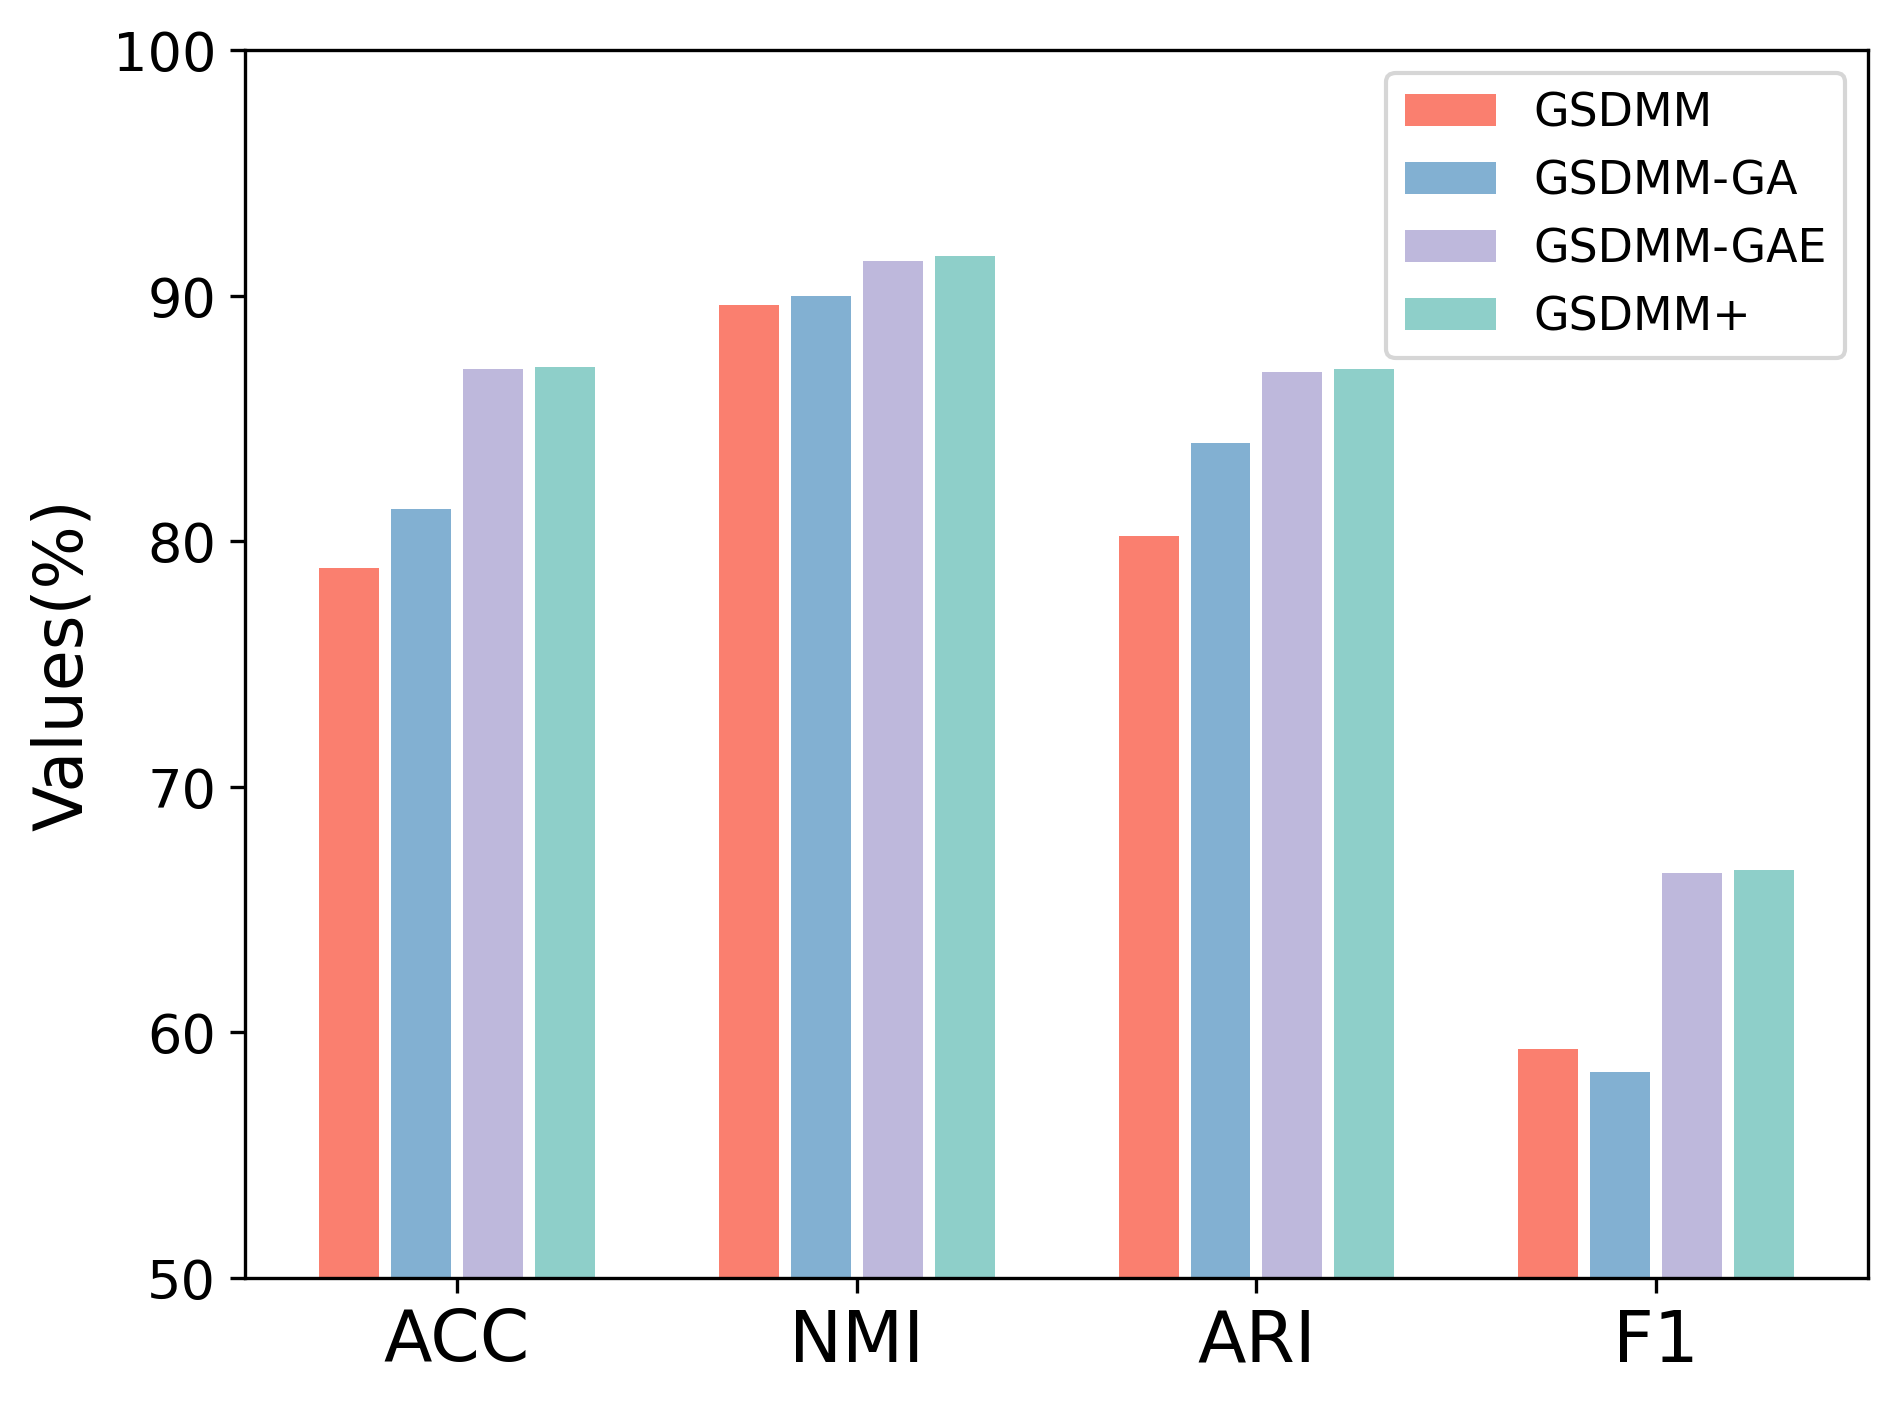
\includegraphics[width=\linewidth]{figure/Tweet_ablation.png}
        \centerline{(a) Tweet}
    \end{minipage}
    \hfill
    \begin{minipage}[t]{0.23\textwidth}
        \centering
        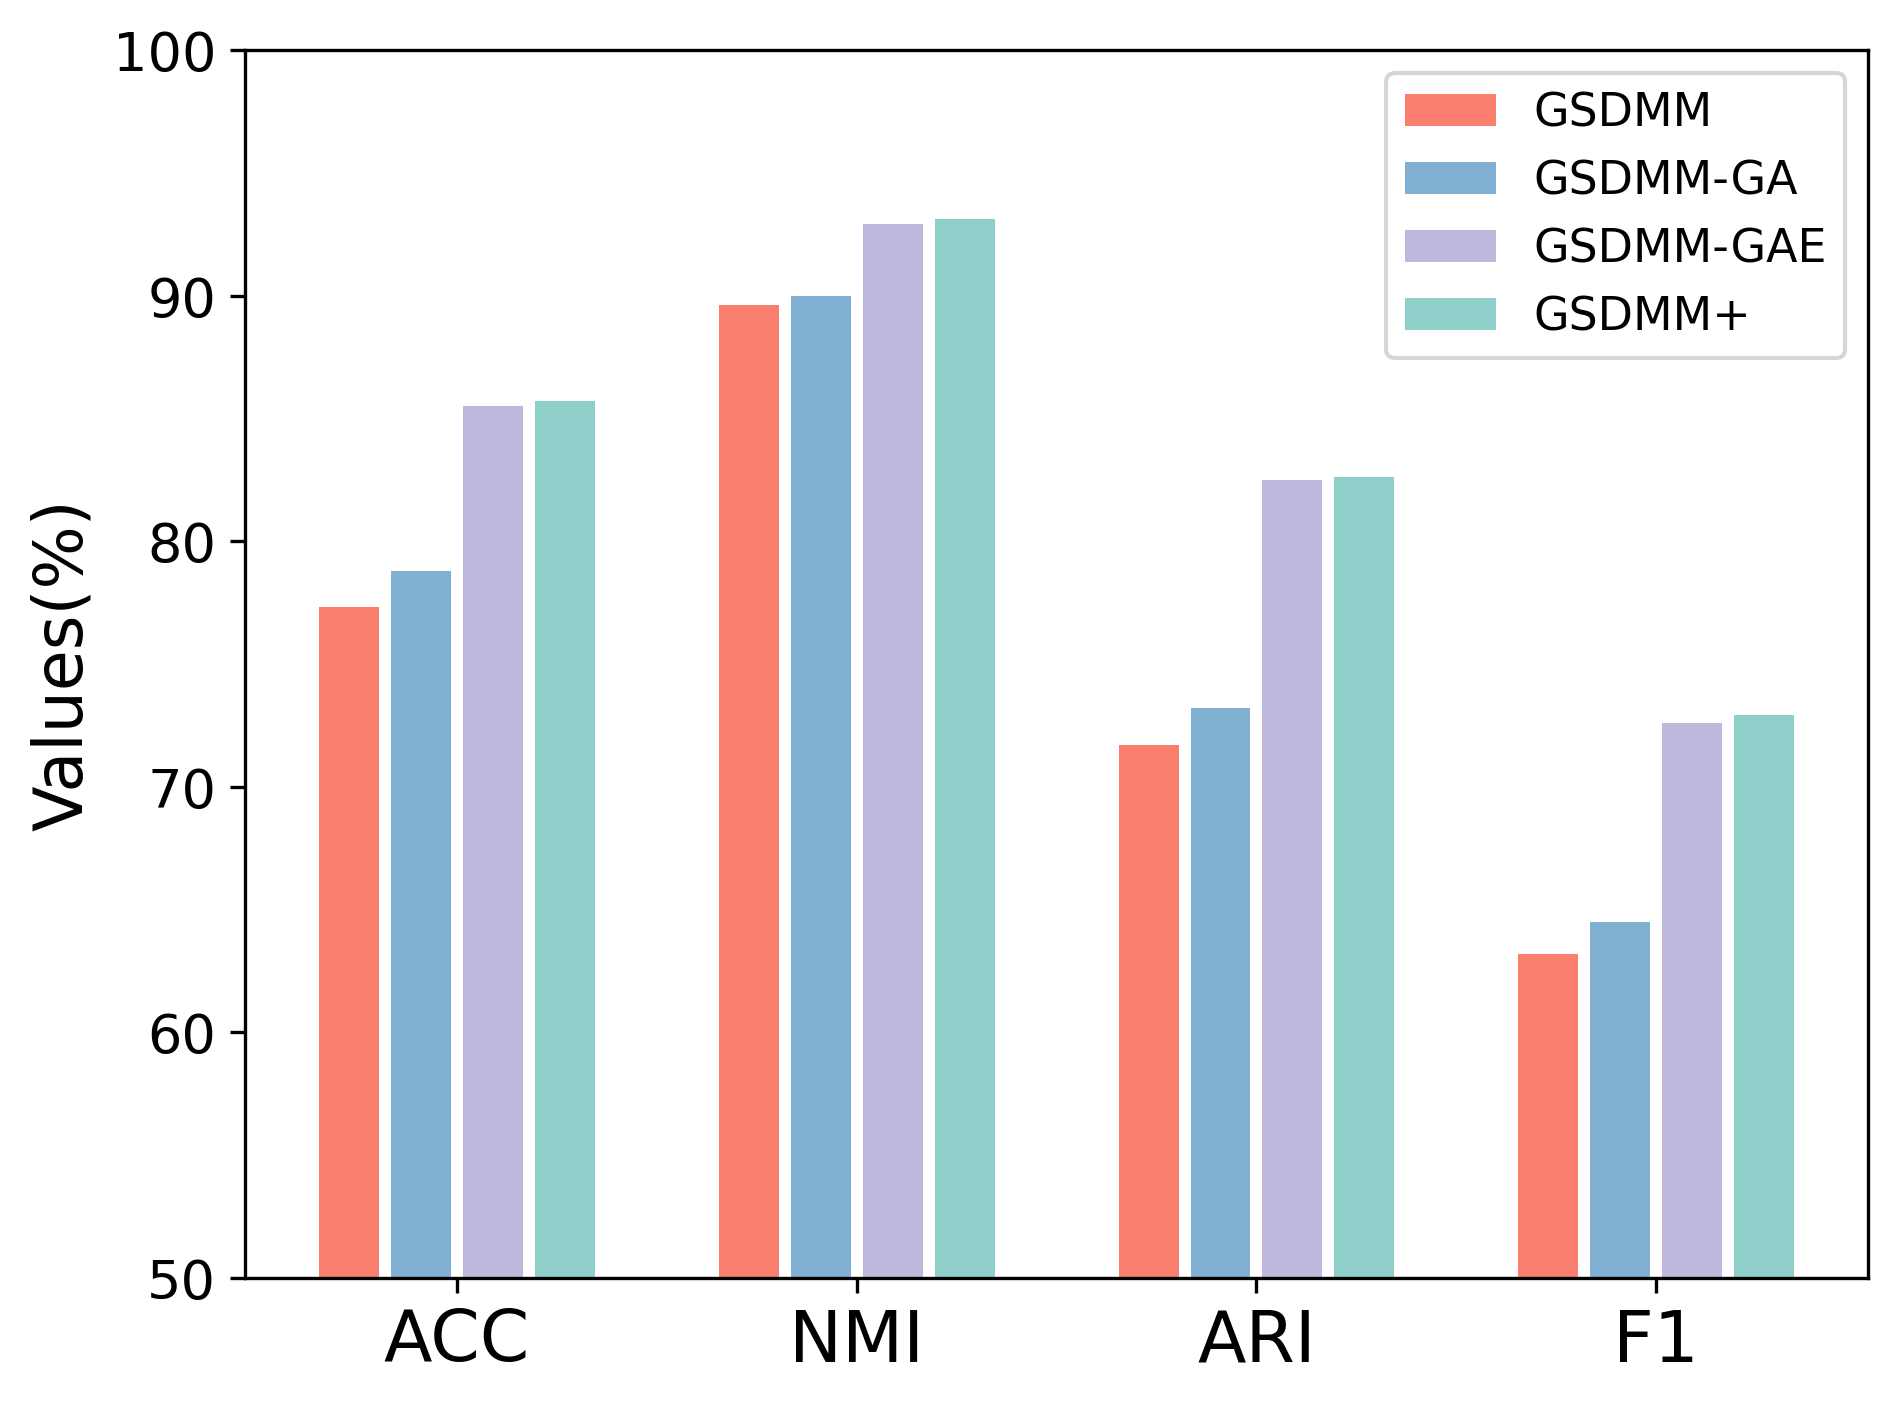
\includegraphics[width=\linewidth]{figure/S_ablation.png}
        \centerline{(b) News-S}
    \end{minipage}
    \hfill
    \begin{minipage}[t]{0.23\textwidth}
        \centering
        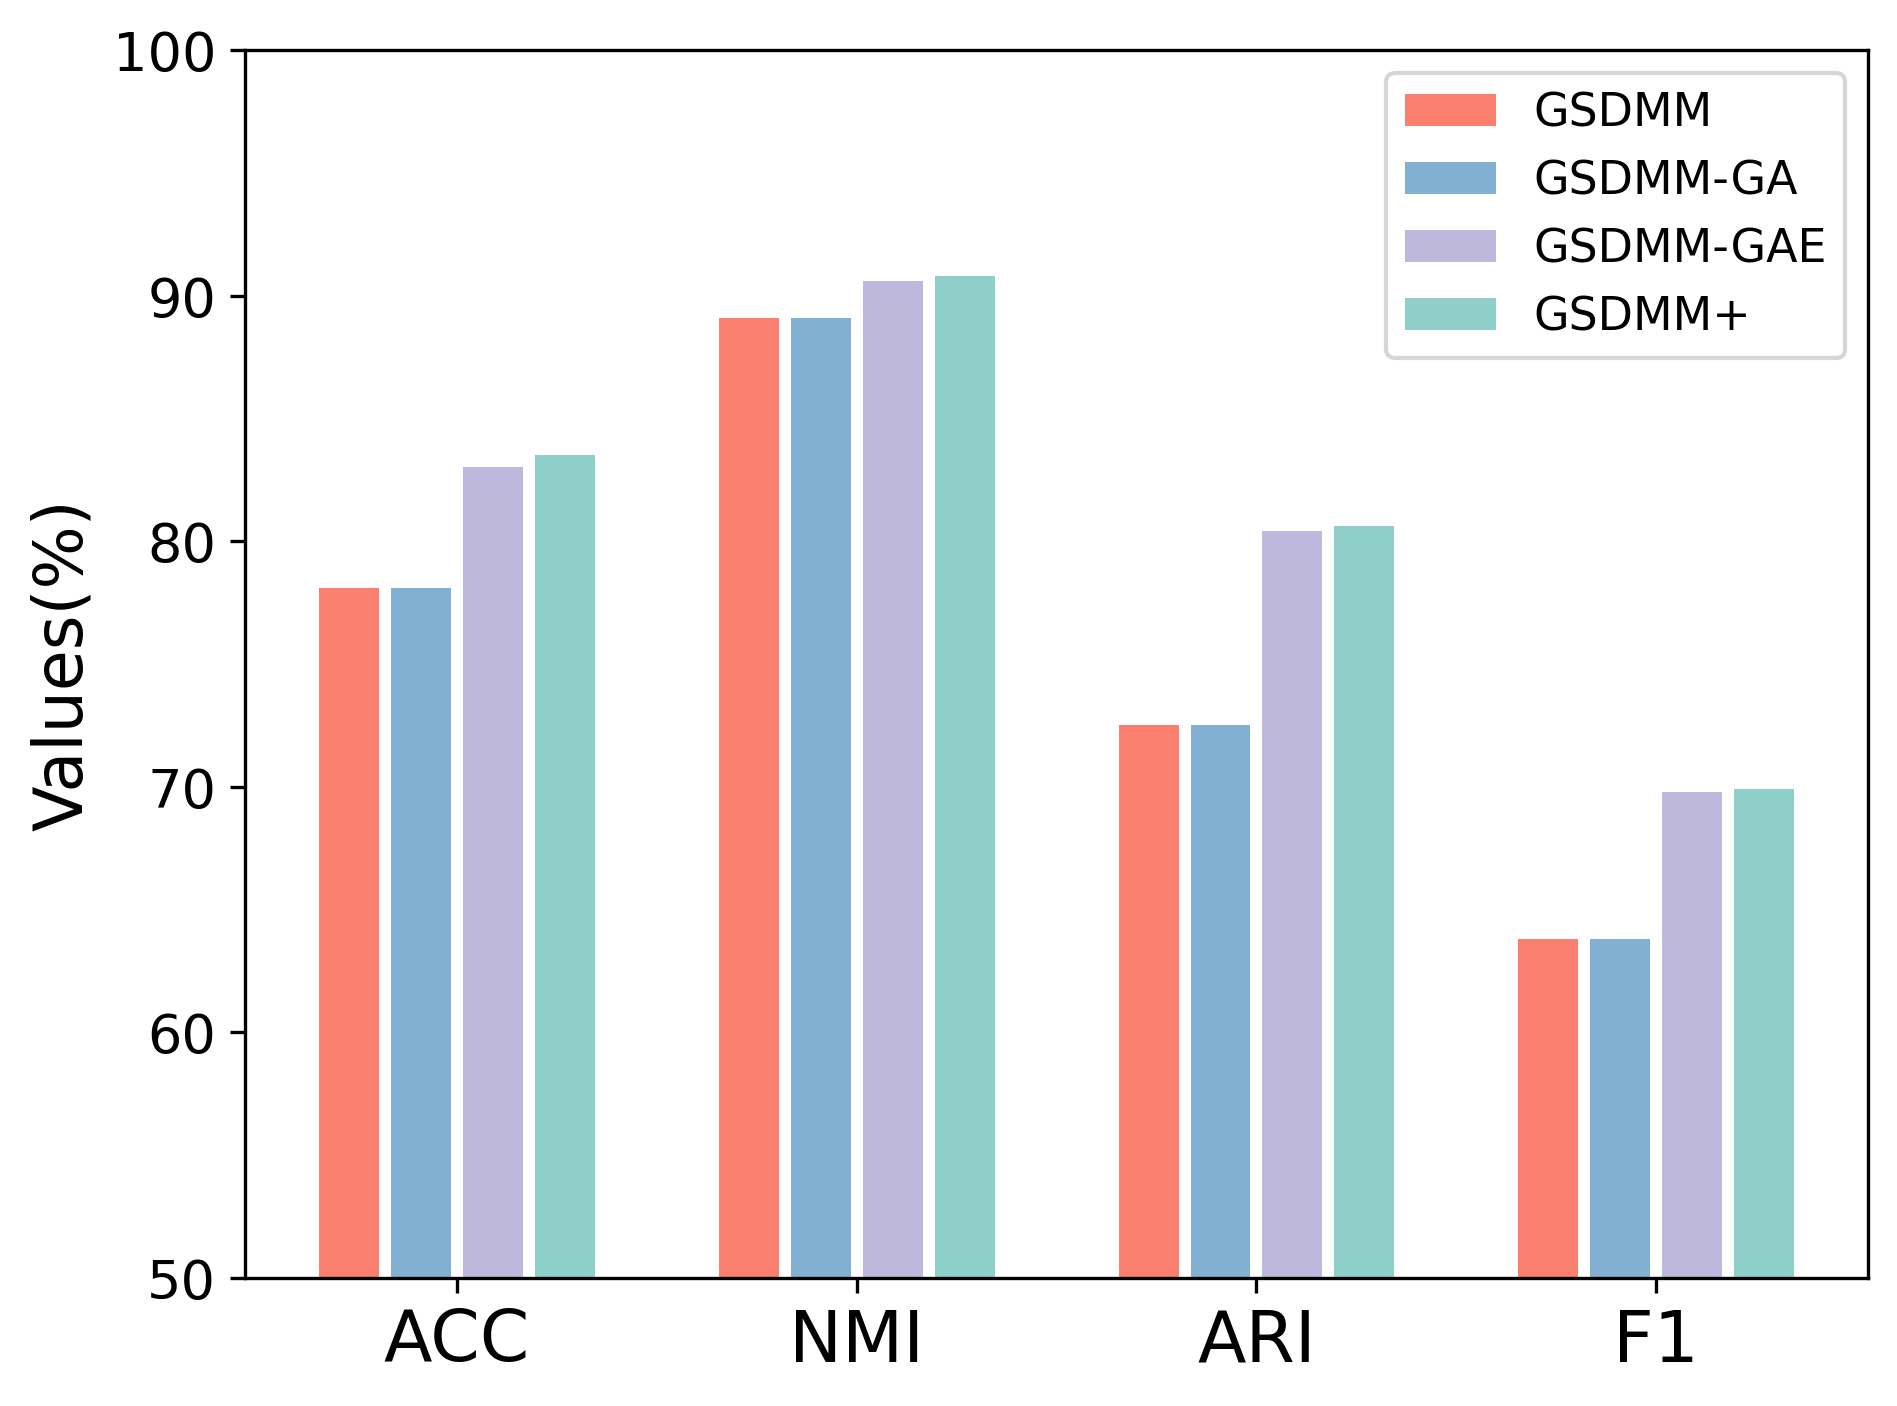
\includegraphics[width=\linewidth]{figure/T_ablation.png}
        \centerline{(c) News-T}
    \end{minipage}
    \hfill
    \begin{minipage}[t]{0.23\textwidth}
        \centering
        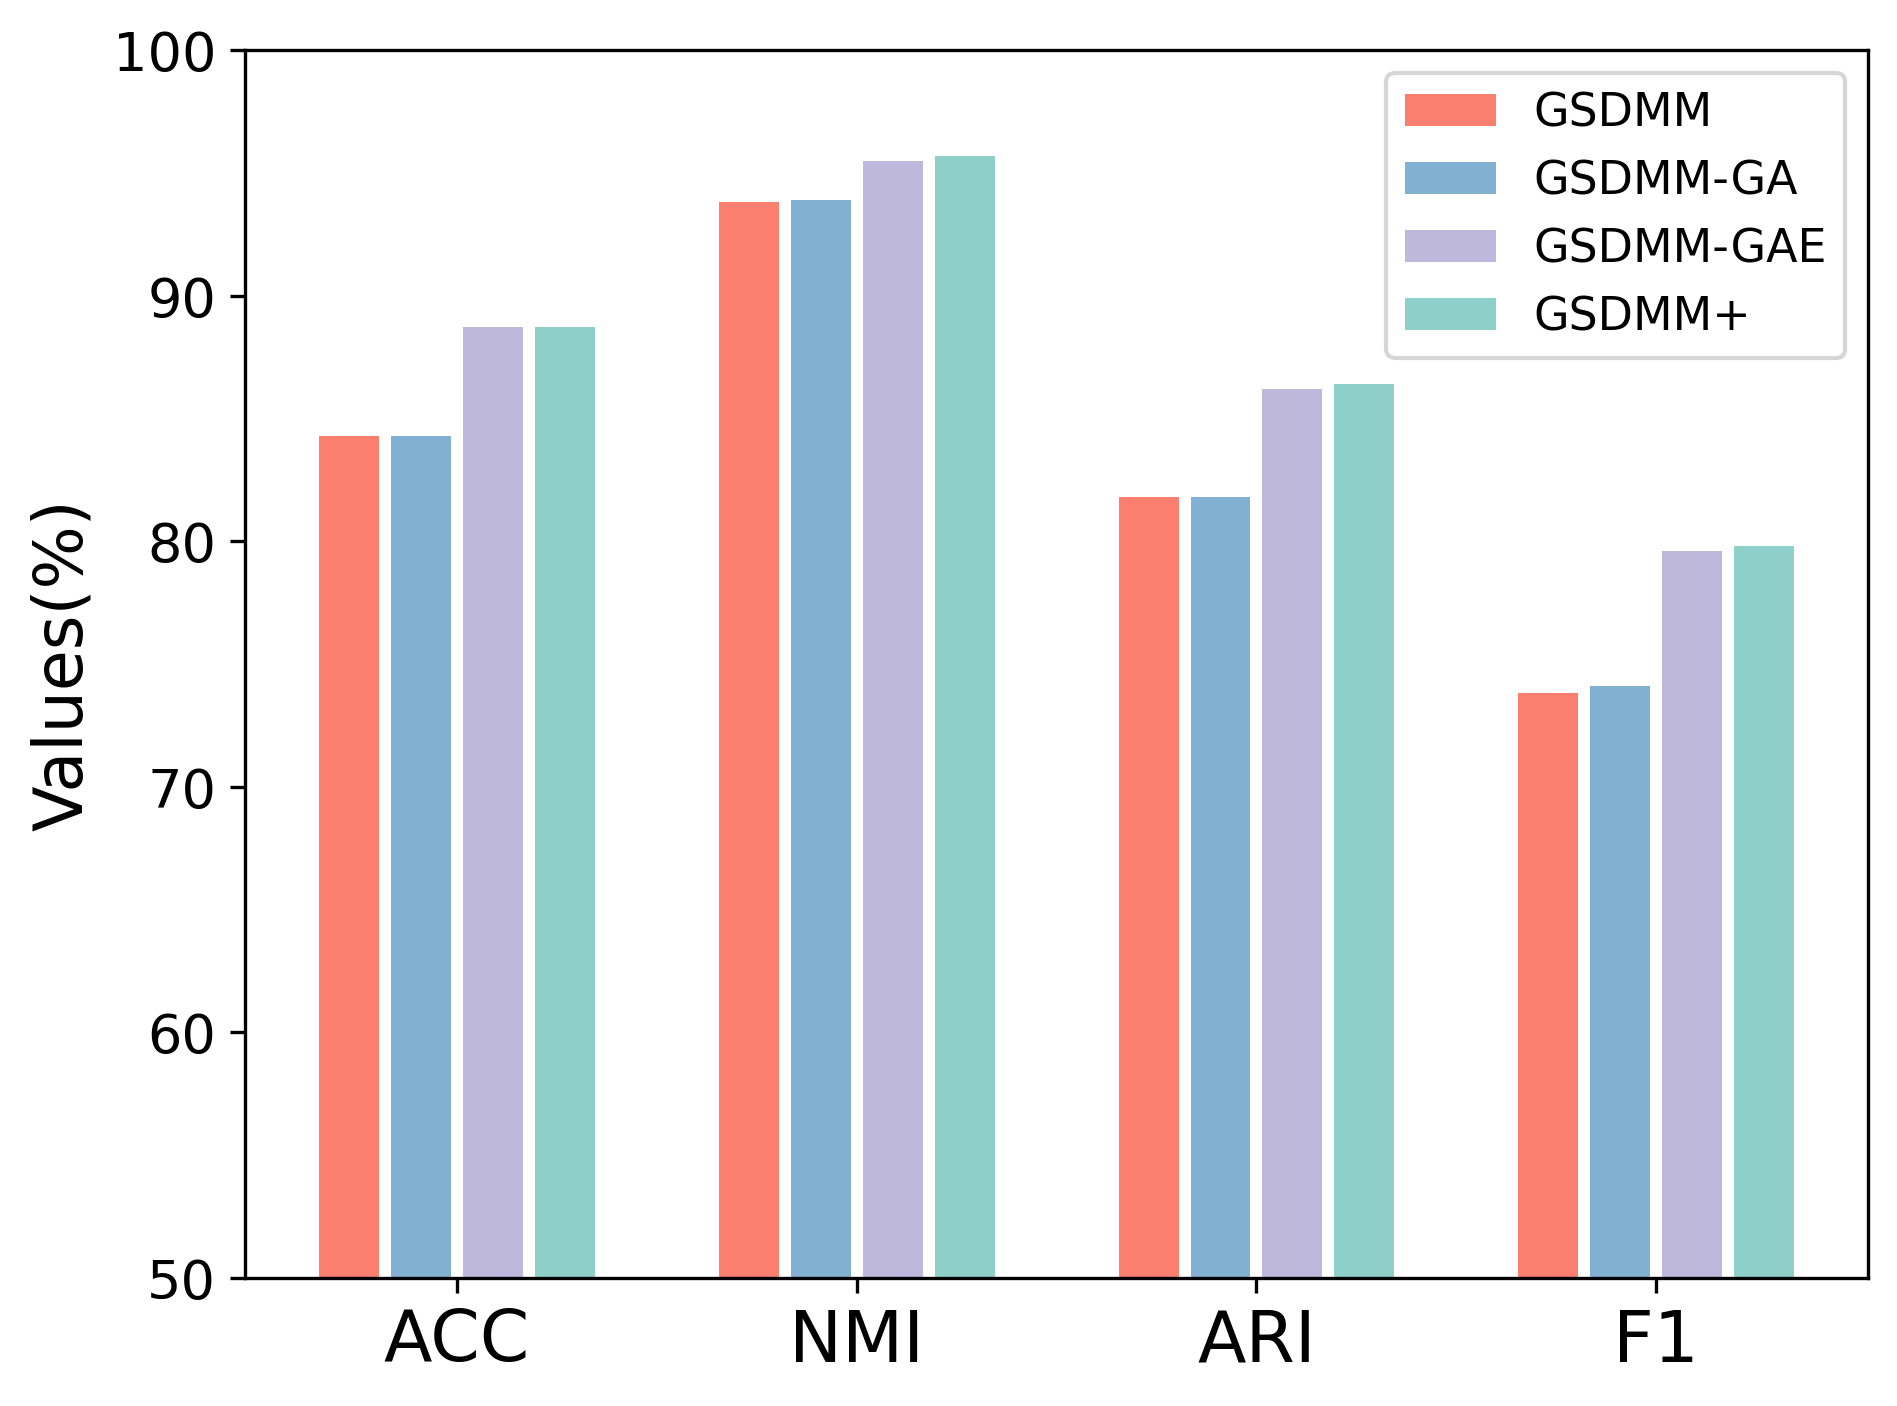
\includegraphics[width=\linewidth]{figure/TS_ablation.png}
        \centerline{(d) News-TS}
    \end{minipage}
\caption{Performance comparison of different module settings for clustering.}
\label{module_Comparison}
\end{figure*}

This section delves into how the proposed designs adjust cluster granularity and improve clustering performance in \sysname{}. Figure~\ref{module_Comparison} presents a comparison of clustering performance under four module settings:
\begin{itemize}
    \item GSDMM: The collapsed Gibbs sampling algorithm for the Dirichlet Multinomial Mixture model.
    \item GSDMM-GA: The method incorporates the granularity adjustment into GSDMM algorithm.
    \item GSDMM-GAE: The method employs entropy-based word weighting and adjusts granularity through cluster merging.
    \item \sysname{}: Our method consists of three modules: adaptive clustering initialization, entropy-based word weighting, and granularity adjustment with cluster merging.
\end{itemize}
Figure~\ref{module_Comparison} presents the ablation studies of the proposed \sysname{} on four datasets, demonstrating consistent and substantial improvements across all metrics.

From the figures, we observe that: 1) In the Tweet and News-S datasets, cluster merging enhances clustering performance by refining the number of clusters. This demonstrates the effectiveness of granularity adjustment in clustering. 2) Across all datasets, our method, which employs entropy-based word weighting and granularity adjustment with cluster merging, significantly improves clustering performance. Entropy-based word weighting refines cluster granularity, enabling the extraction of more fine-grained information. Granularity adjustment determines a reasonable number of clusters, ultimately achieving optimal performance and surpassing methods that rely on text embeddings. 3) Using only entropy-based word weighting to refine cluster granularity creates a discrepancy between the number of clusters and the true number of categories. Without fine-grained adjustment, clustering performance deteriorates significantly. Therefore, this scenario is not included in the presented figures.

% AVI provides a stable starting point, DMM-Entropy refines word-level representations to emphasize critical features, and SCM dynamically adjusts the clustering structure to approach the true underlying categories. Together, these methods enhance the performance of the DMM algorithm, achieving faster convergence, better clustering accuracy, and greater robustness across datasets.

% \begin{table}[htbp]
% \centering
% \caption{Performance Comparison of Different Module Settings for Clustering on Tweet and News-TS Datasets}
% \setlength{\tabcolsep}{6pt}
% \small
% \begin{tabular}{c|c|c|c|c}
% \hline
% \textbf{Dataset} & \textbf{Metric} & \textbf{DMM} & \textbf{DMM+SCM} & \textbf{\sysname{}} \\ \hline
% \multirow{4}{*}{Tweet} & ACC  & 0.789$\pm$0.022 & 0.813$\pm$0.030 & \textbf{0.870\(\pm\)0.011} \\ 
%                       & NMI  & 0.896$\pm$0.005 & 0.900$\pm$0.009 & \textbf{0.914\(\pm\)0.006} \\
%                       & ARI  & 0.802$\pm$0.032 & 0.840$\pm$0.029 & \textbf{0.869\(\pm\)0.010} \\
%                       & F1   & 0.593$\pm$0.026 & 0.584$\pm$0.032 & \textbf{0.665\(\pm\)0.025} \\ \hline
% \multirow{4}{*}{News-T} & ACC  & 0.781$\pm$0.018 & 0.781$\pm$0.018 & \textbf{0.830\(\pm\)0.009} \\ 
%                       & NMI  & 0.891$\pm$0.006 & 0.891$\pm$0.006 & \textbf{0.906\(\pm\)0.003} \\
%                       & ARI  & 0.725$\pm$0.022 & 0.725$\pm$0.022 & \textbf{0.804\(\pm\)0.010} \\
%                       & F1   & 0.638$\pm$0.034 & 0.638$\pm$0.034 & \textbf{0.698\(\pm\)0.016} \\ \hline
% \multirow{4}{*}{News-S} & ACC  & 0.773$\pm$0.023 & 0.788$\pm$0.020 & \textbf{0.855\(\pm\)0.007} \\ 
%                       & NMI  & 0.896$\pm$0.006 & 0.900$\pm$0.005 & \textbf{0.929\(\pm\)0.002} \\
%                       & ARI  & 0.717$\pm$0.032 & 0.732$\pm$0.024 & \textbf{0.825\(\pm\)0.007} \\
%                       & F1   & 0.632$\pm$0.024 & 0.645$\pm$0.019 & \textbf{0.726\(\pm\)0.016} \\ \hline
% \multirow{4}{*}{News-TS} & ACC  & 0.843\(\pm\)0.016 & 0.843\(\pm\)0.017 & \textbf{0.887\(\pm\)0.005} \\ 
%                       & NMI  & 0.938\(\pm\)0.004 & 0.939\(\pm\)0.005 & \textbf{0.955\(\pm\)0.002} \\
%                       & ARI  & 0.818\(\pm\)0.022 & 0.818\(\pm\)0.017 & \textbf{0.862\(\pm\)0.006} \\
%                       & F1   & 0.738\(\pm\)0.012 & 0.741\(\pm\)0.028 & \textbf{0.796\(\pm\)0.016} \\ \hline

% \end{tabular}
% \label{module_Comparison}
% \end{table}

% \begin{figure}[!t]
% \centering
% \begin{minipage}{0.49\linewidth}
% % \centerline{Positive Sample Pairs}
% \centerline{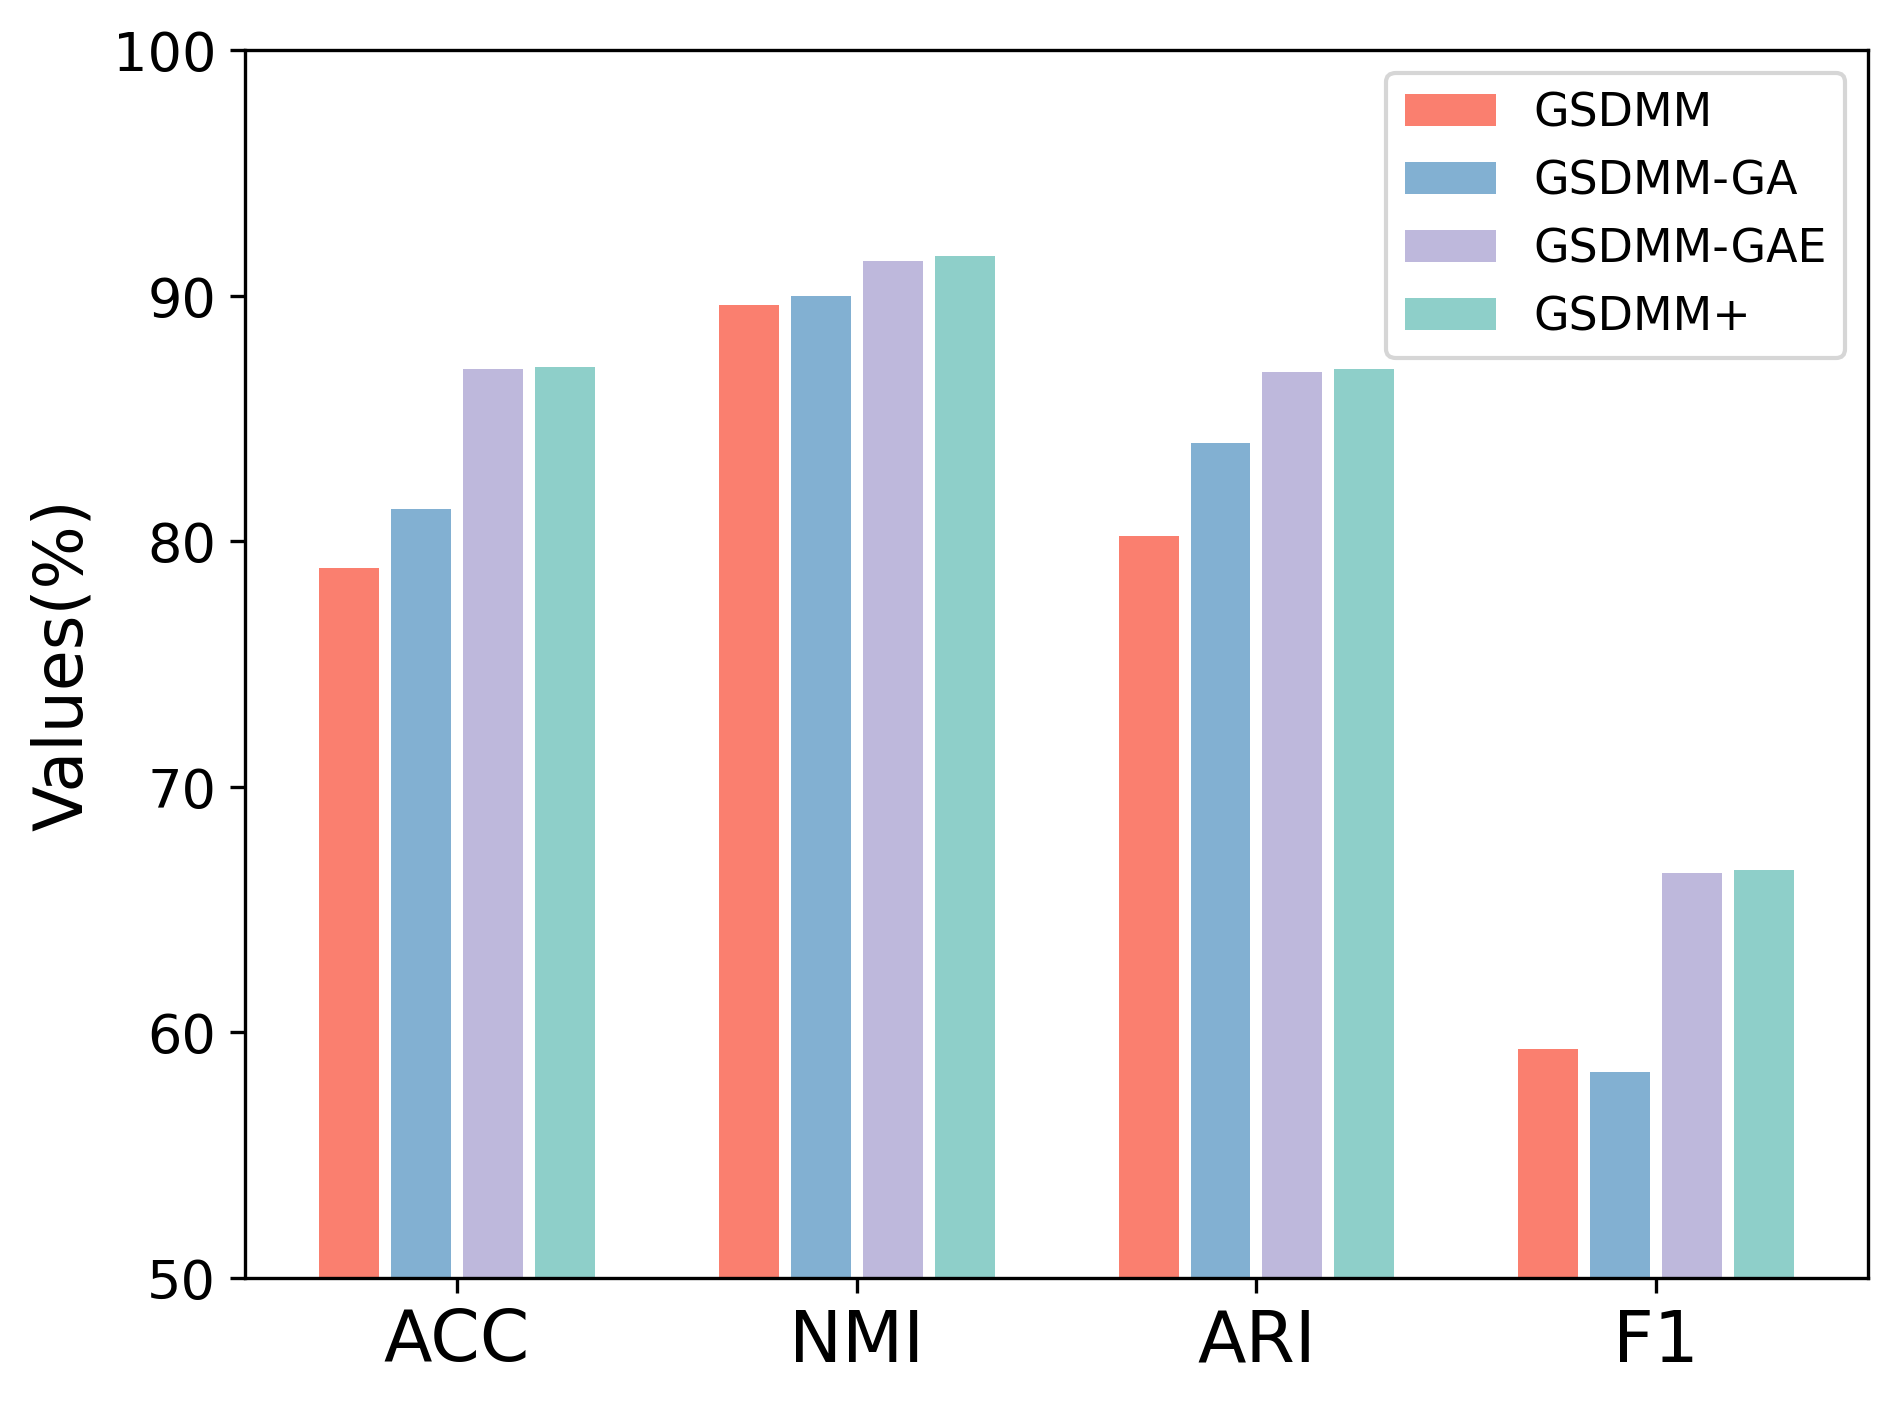
\includegraphics[width=0.98\textwidth]{figure/Tweet_ablation.png}}
% \centerline{(a) Tweet}
% \centerline{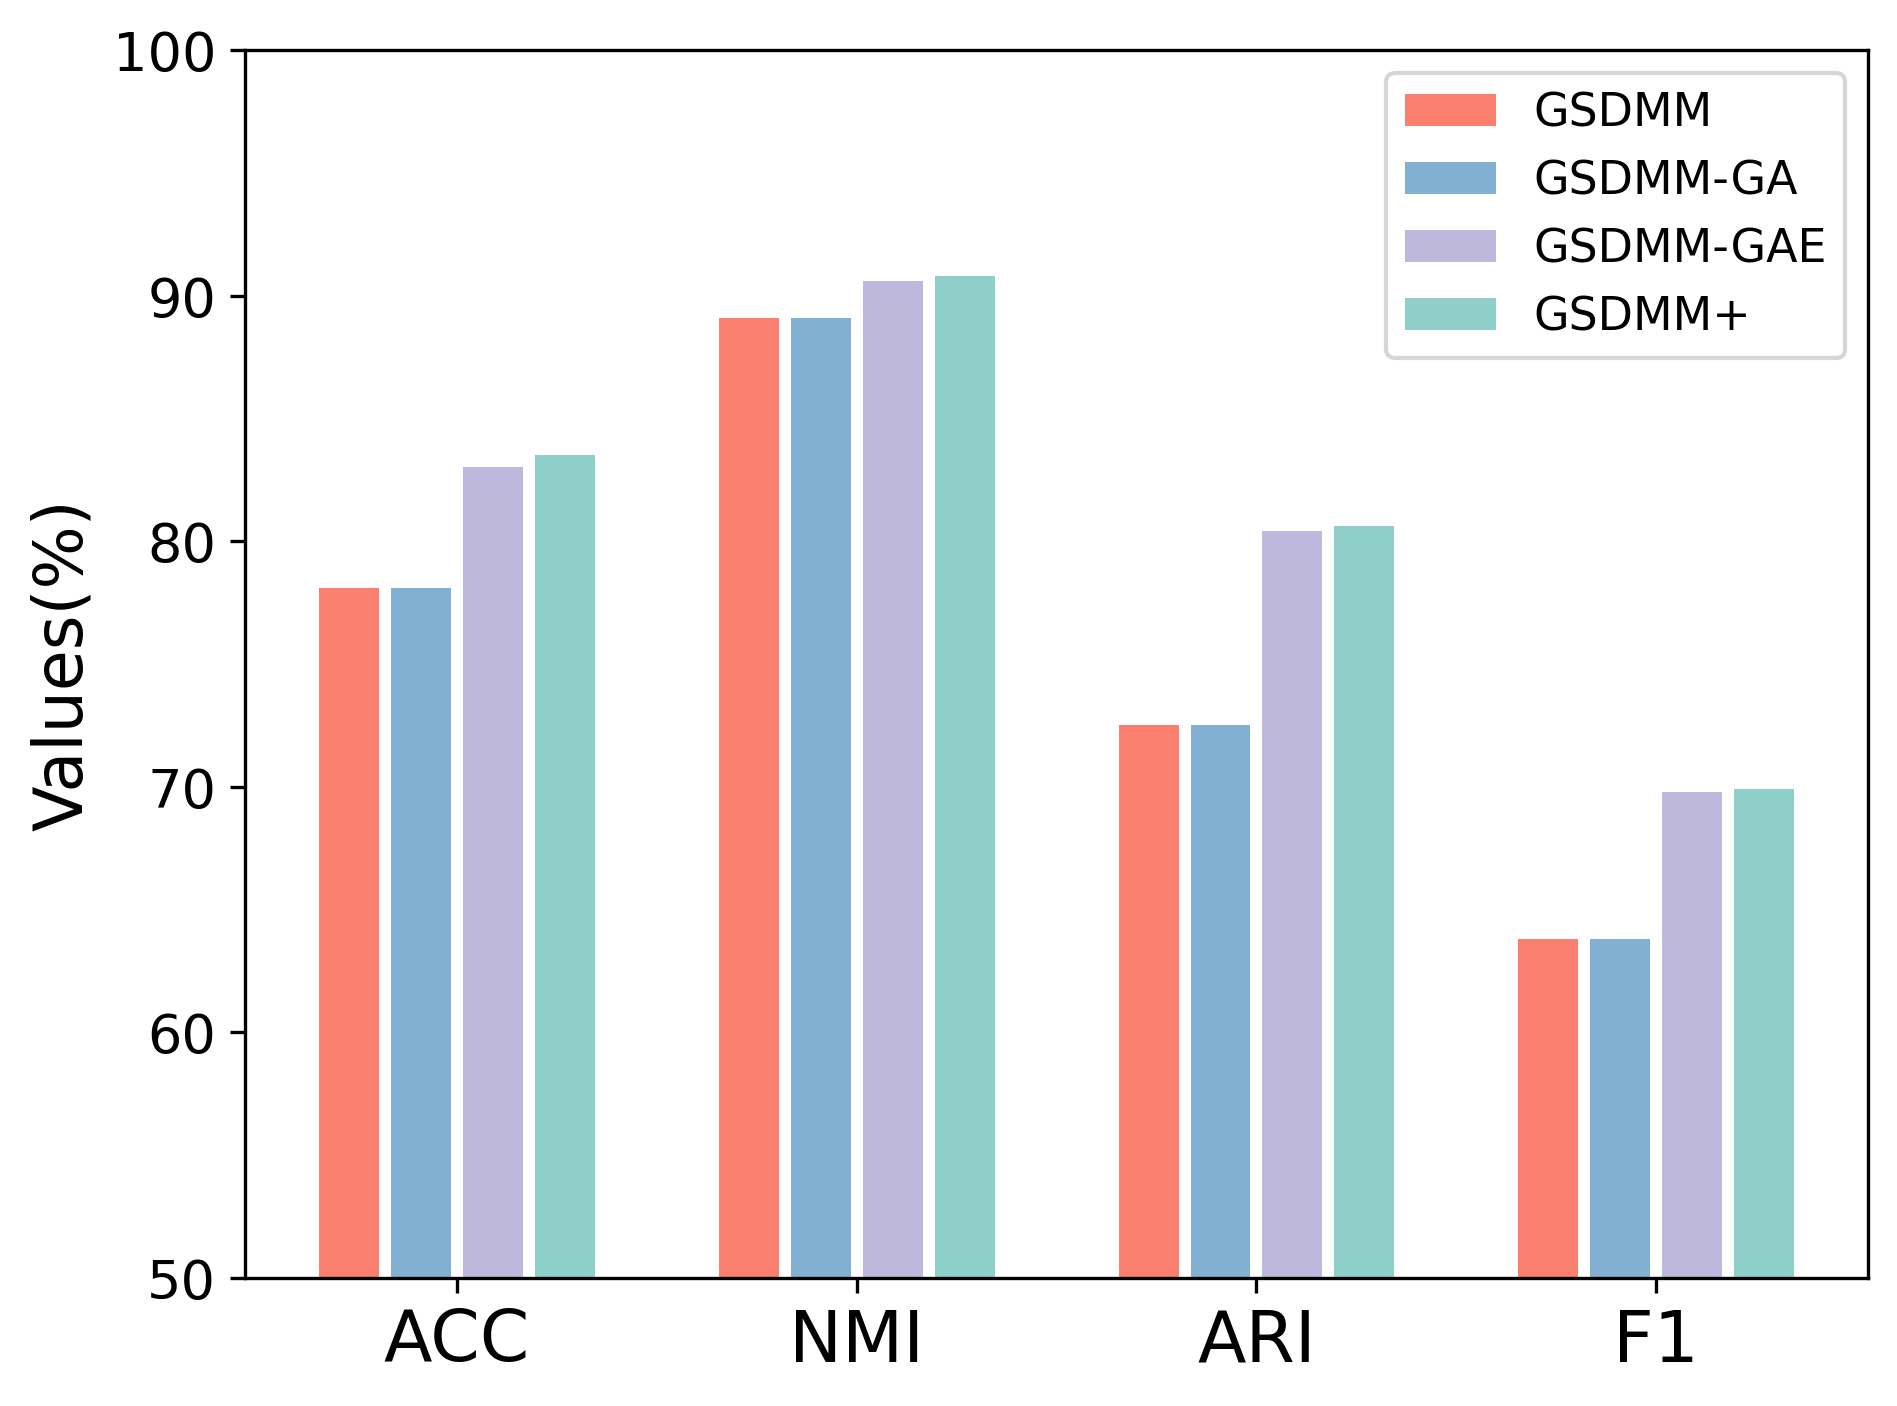
\includegraphics[width=0.98\textwidth]{figure/T_ablation.png}}
% \centerline{(c) News-T}
% \end{minipage}
% \begin{minipage}{0.49\linewidth}
% % \centerline{Negative Sample Pairs}
% \centerline{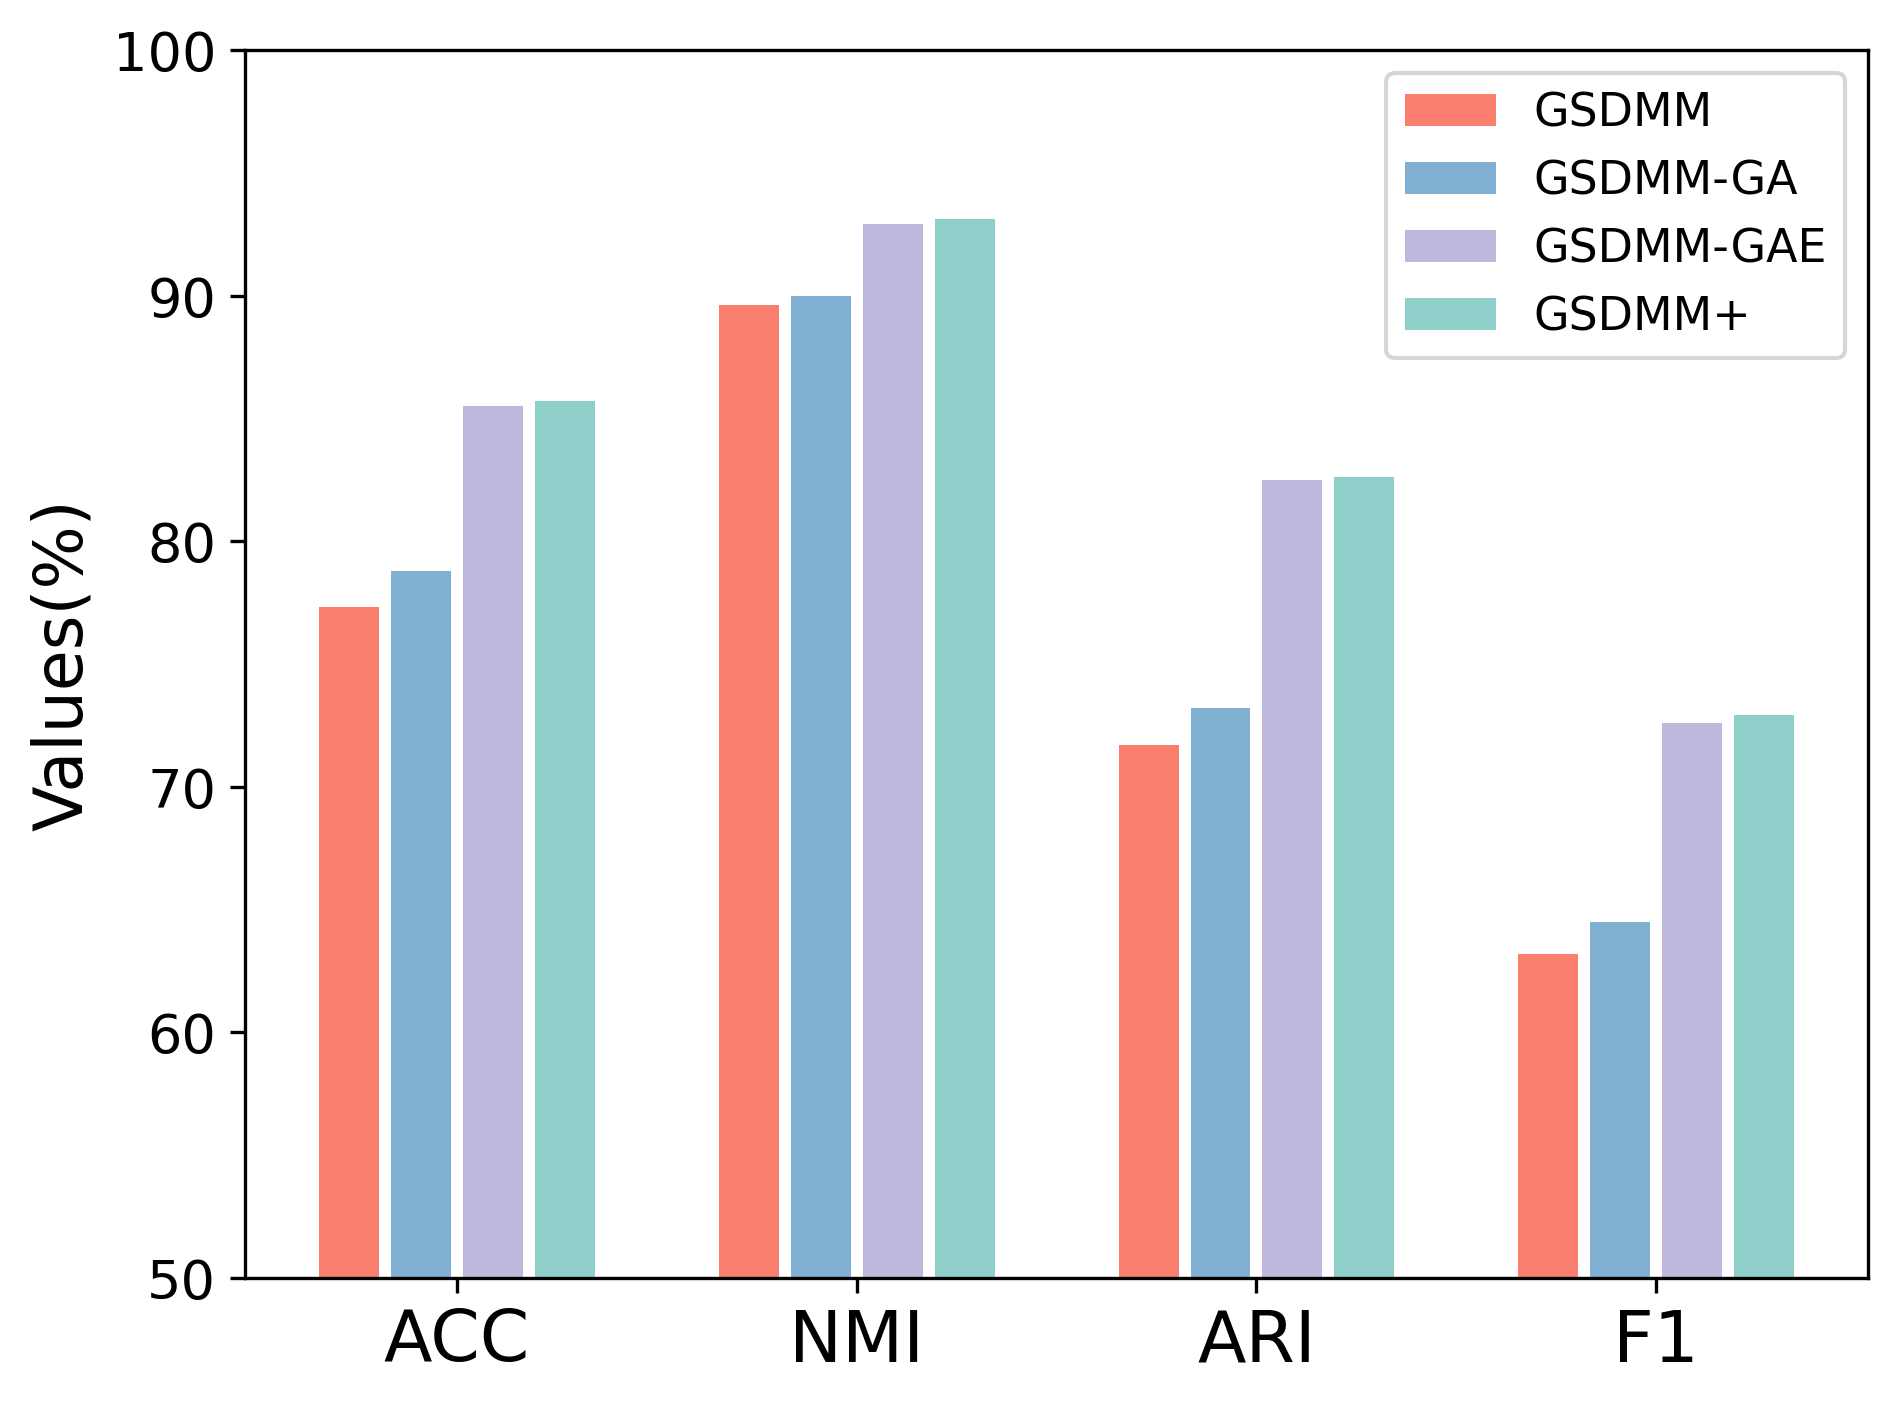
\includegraphics[width=0.98\textwidth]{figure/S_ablation.png}}
% \centerline{(b) News-S}
% \centerline{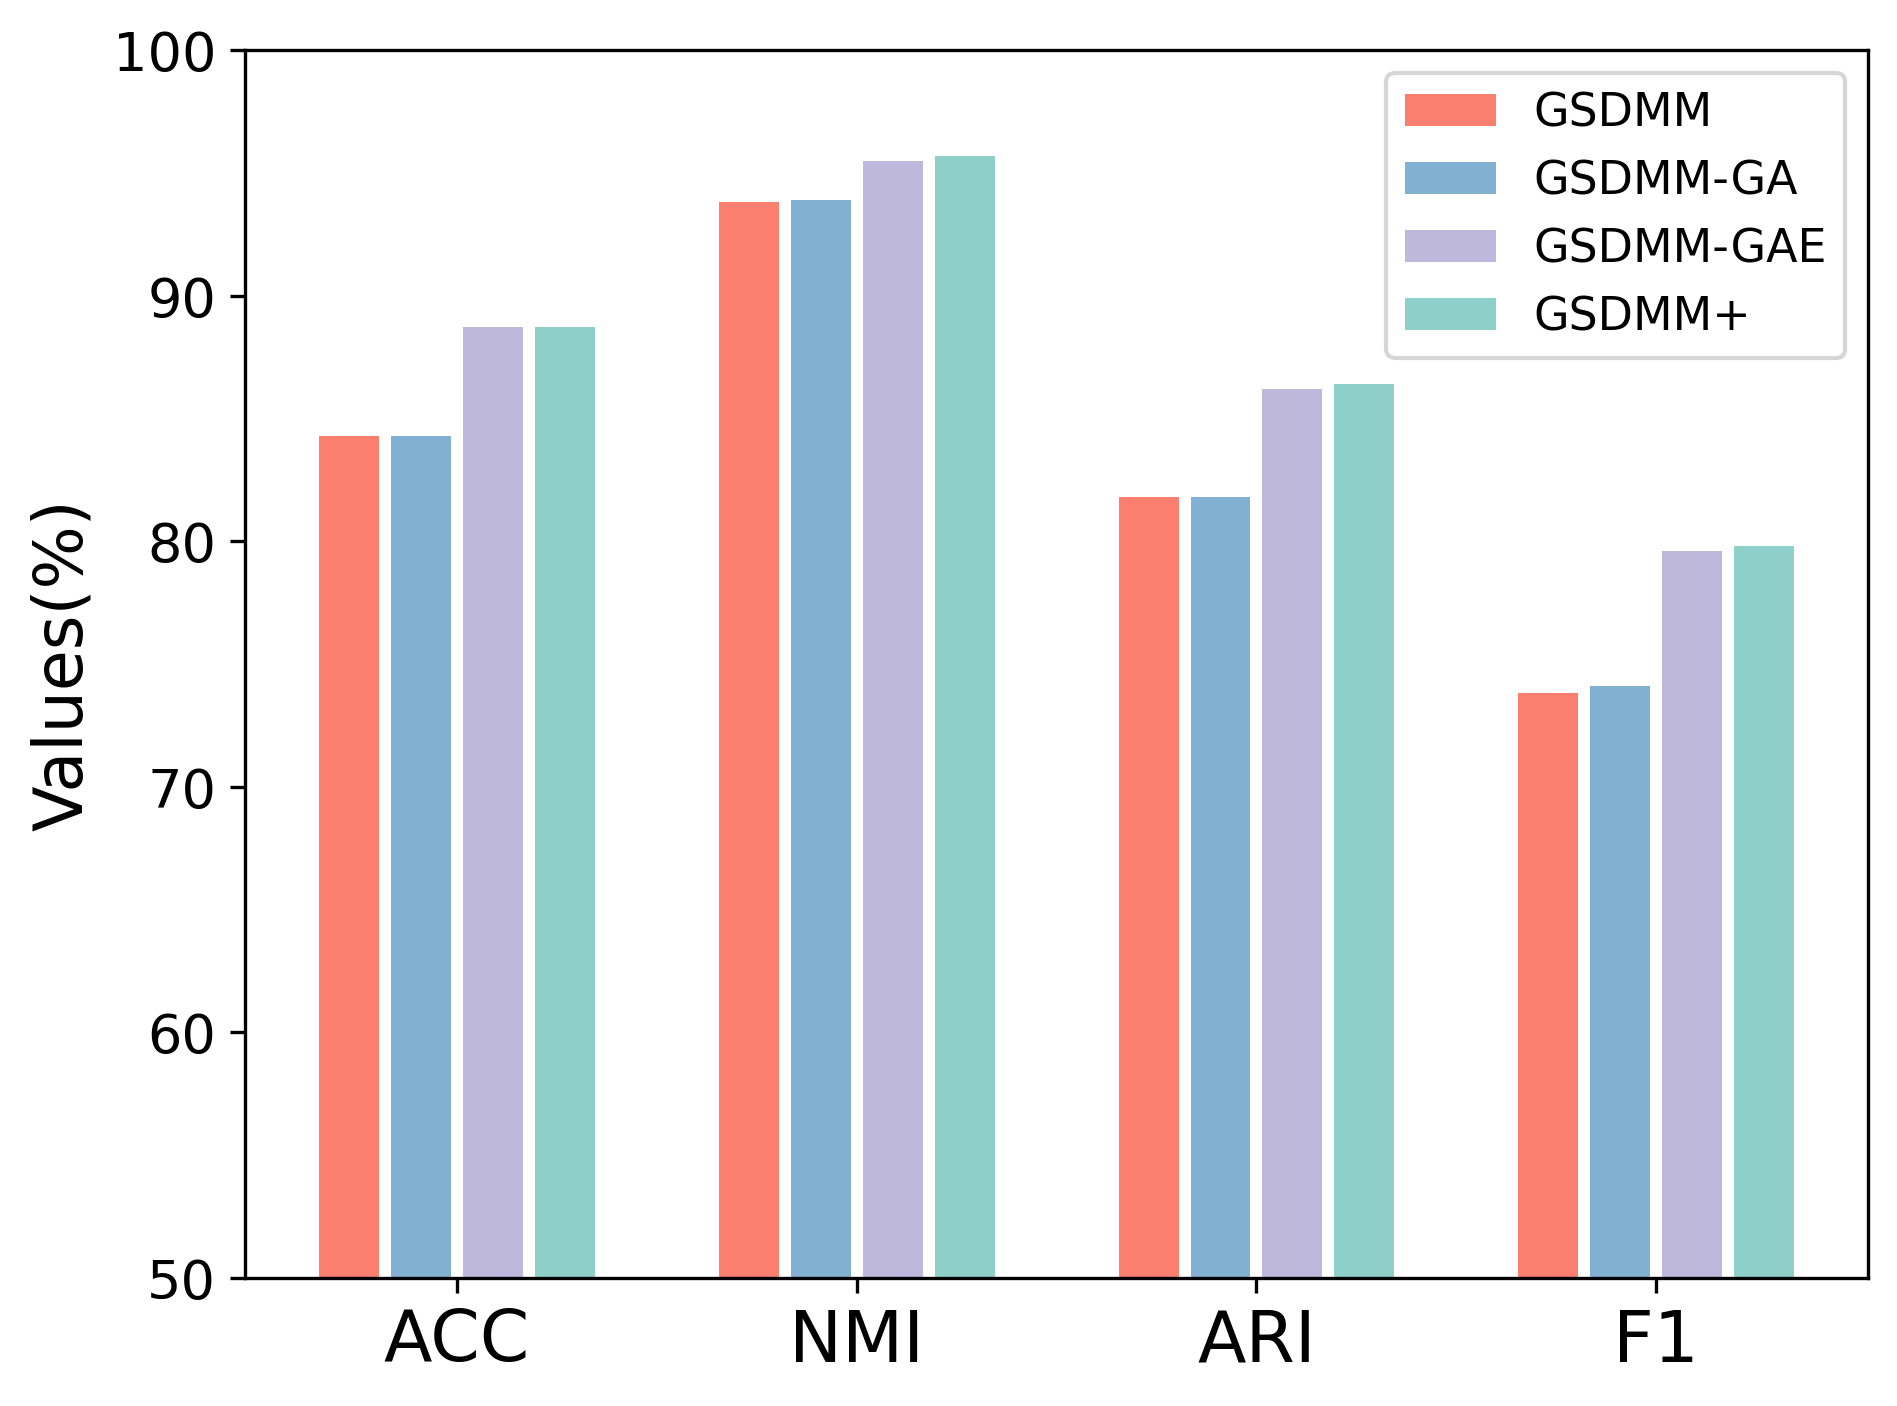
\includegraphics[width=0.98\textwidth]{figure/TS_ablation.png}}
% \centerline{(d) News-TS}
% \end{minipage}
% \caption{Performance comparison of different module settings for clustering}
% \label{module_Comparison}
% \end{figure}

\subsubsection{Adaptive Clustering Initialization}
To effectively demonstrate the necessity and effectiveness of the adaptive clustering initialization module, we present experimental results conducted on two distinct datasets: Tweet and News-TS. 

\begin{figure}[t]
\centering
\begin{minipage}{0.49\linewidth}
\centerline{\includegraphics[width=0.98\textwidth]{figure/tweet_initK.png}}
\centerline{(a) Tweet}
\end{minipage}
\begin{minipage}{0.49\linewidth}
\centerline{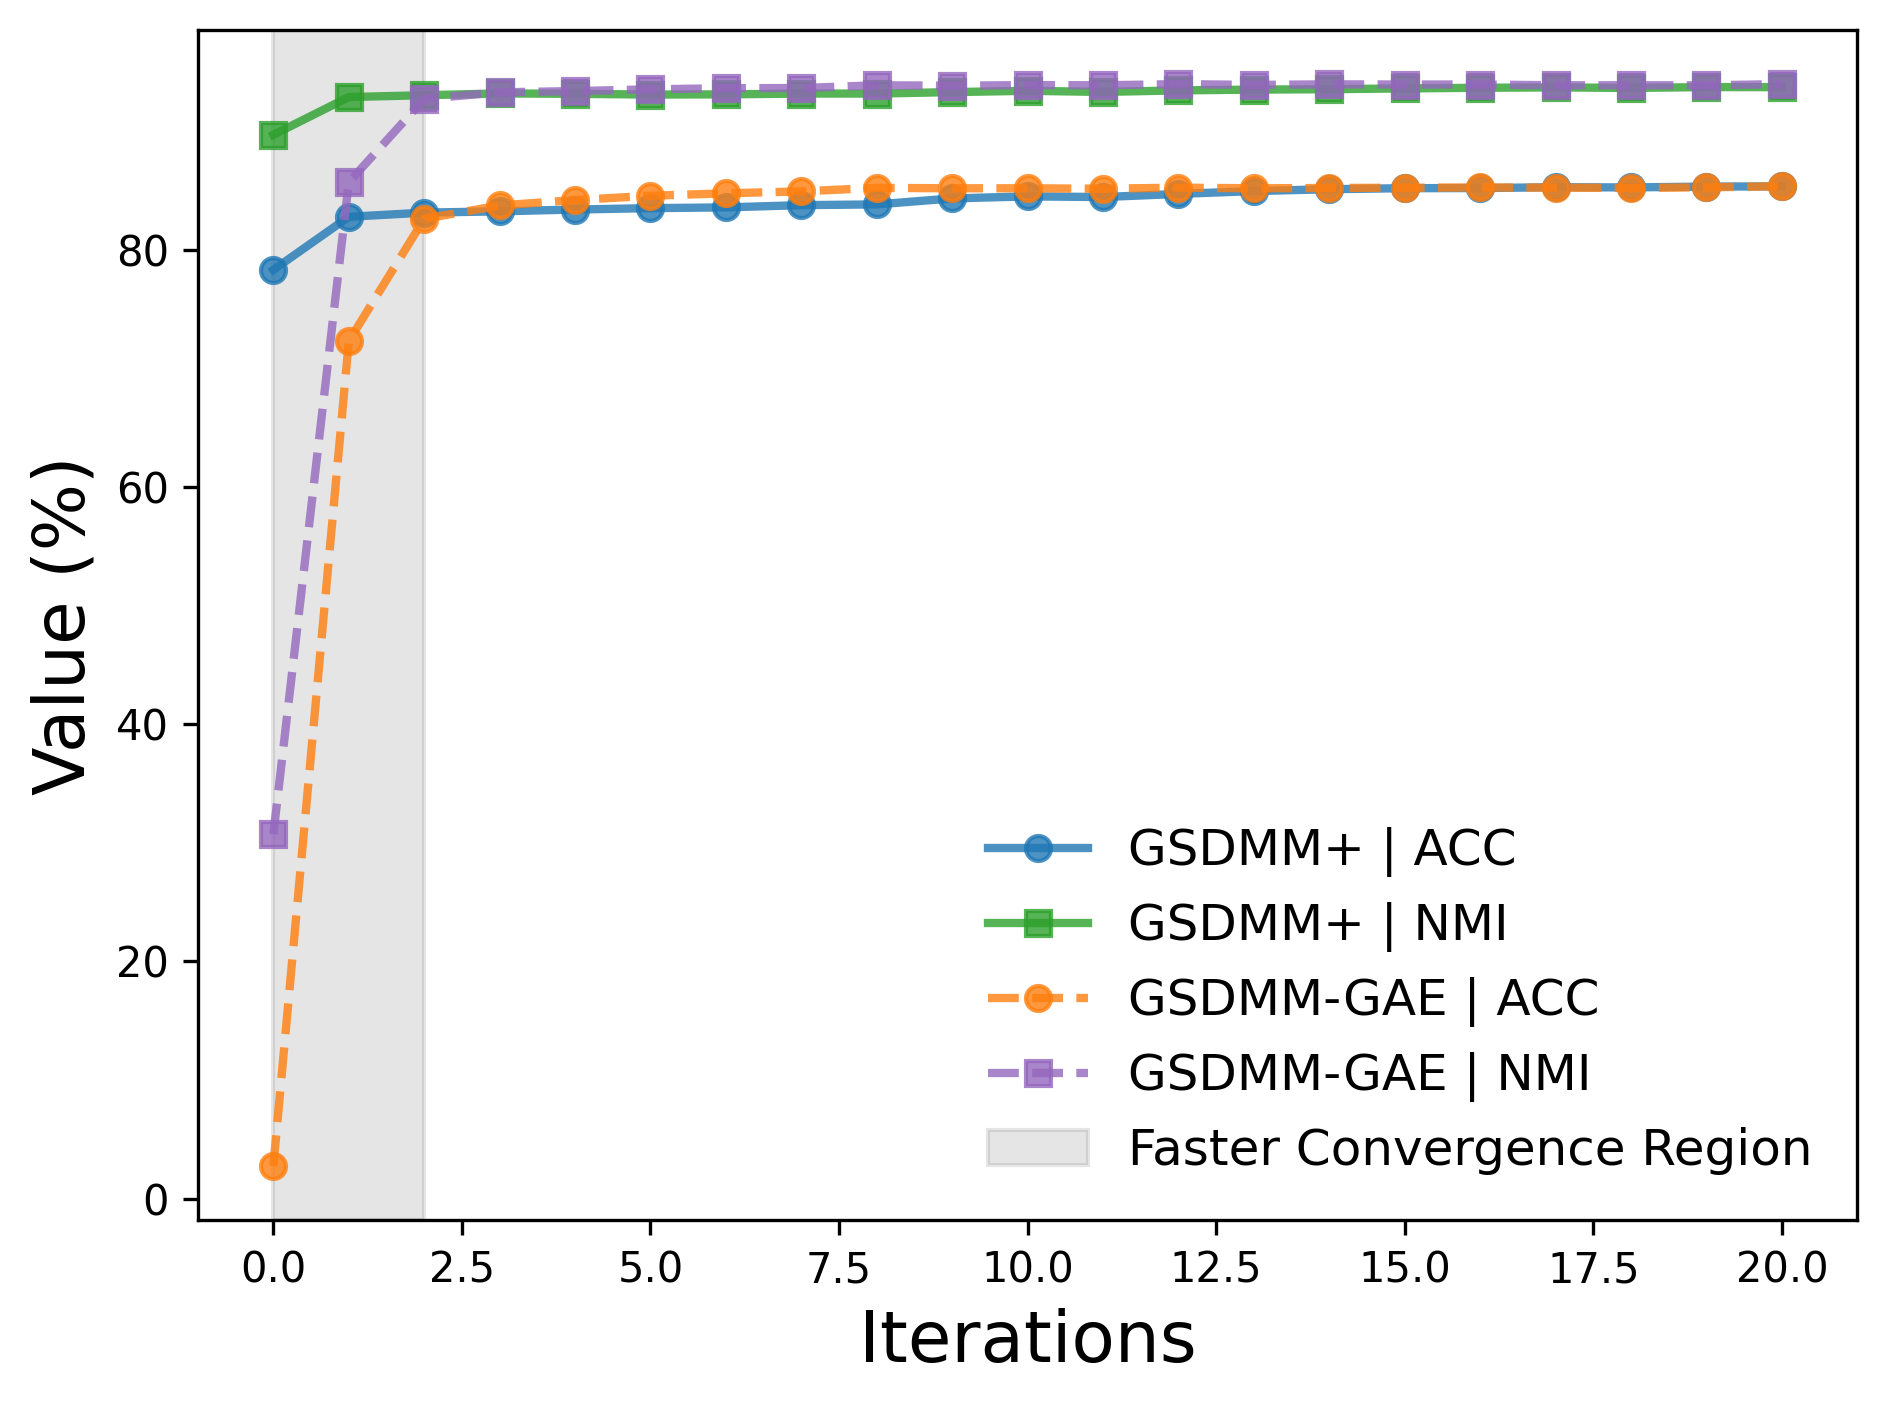
\includegraphics[width=0.98\textwidth]{figure/TS_initK.png}}
\centerline{(b) News-TS}
\end{minipage}
\caption{Comparison of clustering performance using adaptive clustering initialization (\sysname{}) and random initialization (GSDMM-GAE) on the Tweet and News-TS Datasets.}
\label{tweet+TS_initK}
\end{figure}

Figure~\ref{tweet+TS_initK} illustrates the comparative performance of adaptive clustering initialization and random initialization on the Tweet and News-TS datasets, respectively. The results highlight several key observations: 1) Adaptive clustering initialization consistently achieves higher ACC and NMI scores within fewer iterations than random initialization. This indicates that our method facilitates more efficient convergence, reducing the number of iterations required to reach stable and optimal clustering results. 2) Unlike random initialization, which shows significant fluctuations in ACC and NMI scores during the early stages, adaptive clustering initialization maintains a steadier improvement trajectory. It also demonstrates greater stability across iterations, crucial for ensuring reliable clustering outcomes.

The comparison clearly demonstrates that adaptive clustering initialization enhances the efficiency of the clustering process. The \sysname{} algorithm achieves faster convergence and improves performance in early iterations by leveraging a structured initialization strategy. 

% This advantage is particularly valuable for large-scale and noisy datasets like Tweets, where computational efficiency and stability are critical.

\subsubsection{Entropy-based Word Weighting}
Unlike the original DMM model, which assigns equal importance to all words and struggles to adjust the hyper-parameter $\beta$ to obtain an appropriate number of clusters, our method leverages word entropy to represent word importance in clustering. This enables the model to generate finer-grained clusters and enhances its ability to capture deeper insights from textual content.

\begin{table}[htbp]
\caption{Top 20 (left) and bottom 20 (right) items by entropy on Tweet.}
\begin{minipage}{0.45\linewidth}
    \centering
    \renewcommand{\arraystretch}{1.1} % 调整行间距
    \setlength{\tabcolsep}{7pt} % 调整列间距（默认是6pt）
    \label{tab:top20}
    \begin{tabular}{ccc}
    \toprule
    \textbf{Rank} & \textbf{Word} & \textbf{Entropy} \\
    \midrule
    1  & news     & 1.0000 \\
    2  & will     & 0.8436 \\
    3  & time     & 0.8415 \\
    4  & today    & 0.8128 \\
    5  & day      & 0.7446 \\
    6  & report   & 0.7335 \\
    7  & blog     & 0.7280 \\
    8  & post     & 0.7271 \\
    9  & ap       & 0.7121 \\
    10 & year     & 0.7097 \\
    11 & well     & 0.7084 \\
    12 & good     & 0.7002 \\
    13 & reuters  & 0.6985 \\
    14 & state    & 0.6903 \\
    15 & help     & 0.6730 \\
    16 & going    & 0.6683 \\
    17 & great    & 0.6676 \\
    18 & set      & 0.6670 \\
    19 & read     & 0.6605 \\
    20 & gt       & 0.6576 \\
    \bottomrule
    \end{tabular}
\end{minipage}
\hspace{0.4cm}
\begin{minipage}{0.45\linewidth}
    \centering
    \renewcommand{\arraystretch}{1.1} % 调整行间距
    \setlength{\tabcolsep}{7pt} % 调整列间距（默认是6pt）
    \label{tab:bottom20}
    \begin{tabular}{ccc}
    \toprule
    \textbf{Rank} & \textbf{Word} & \textbf{Entropy} \\
    \midrule
    1  & debt        & 2.92e-7 \\
    2  & djokovic    & 2.92e-7 \\
    3  & setting     & 2.92e-7 \\
    4  & emanuel     & 2.92e-7 \\
    5  & starbucks   & 2.92e-7 \\
    6  & rahm        & 2.92e-7 \\
    7  & kardashian  & 2.92e-7 \\
    8  & aid         & 2.92e-7 \\
    9  & iran        & 2.92e-7 \\
    10 & chrysler    & 2.92e-7 \\
    11 & aquarium    & 2.92e-7 \\
    12 & cup         & 2.92e-7 \\
    13 & meat        & 2.92e-7 \\
    14 & obamacare   & 2.92e-7 \\
    15 & eminem      & 2.92e-7 \\
    16 & ballot      & 2.92e-7 \\
    17 & chavez      & 2.92e-7 \\
    18 & swan        & 2.92e-7 \\
    19 & olbermann   & 2.92e-7 \\
    20 & term        & 2.92e-7 \\
    \bottomrule
    \end{tabular}
\end{minipage}
\label{tab:two_side_by_side}
\end{table}

As shown in Table~\ref{tab:two_side_by_side}, the following observations can be made: 1) In our method, although most words retain their information after stop words are removed, experimental analysis reveals significant differences in word importance for cluster formation and variations in the amount of information carried by different words.
2) Words with high entropy exhibit significant non-thematic characteristics, indicating that they are broadly distributed across categories and thus less informative for clustering. Their inclusion may introduce noise, highlighting the importance of identifying and down-weighting such words. In contrast, words with entropy close to zero demonstrate strong thematic relevance and serve as reliable indicators of category membership, making them critical for clustering tasks. Therefore, using entropy is essential for evaluating word-topic relevance.

The visualization of entropy confirms that word importance is not uniform. By leveraging word entropy, we can prioritize low-entropy words for clustering while reducing the impact of high-entropy words. This refinement improves the performance of the GSDMM model, leading to more accurate and meaningful clustering results.

\subsubsection{Granularity Adjustment with Cluster Merging}
In our method, entropy-based word weighting enables the discovery of finer-grained clusters and the uncovering of deeper latent topics, which more accurately capture the inherent semantic structure of the data. However, the mismatch between the number of clusters and the true categories negatively impacts performance. 

To address this issue, we apply granularity adjustment with cluster merging. Specifically, clusters with high similarity are merged, reducing redundancy and progressively refining the clustering structure to better align with the true underlying categories. This technique ensures cluster number alignment while preserving fine-grained information extraction, ultimately achieving superior clustering performance.

\begin{figure}[!t]
\centering
\begin{minipage}{0.49\linewidth}
\centerline{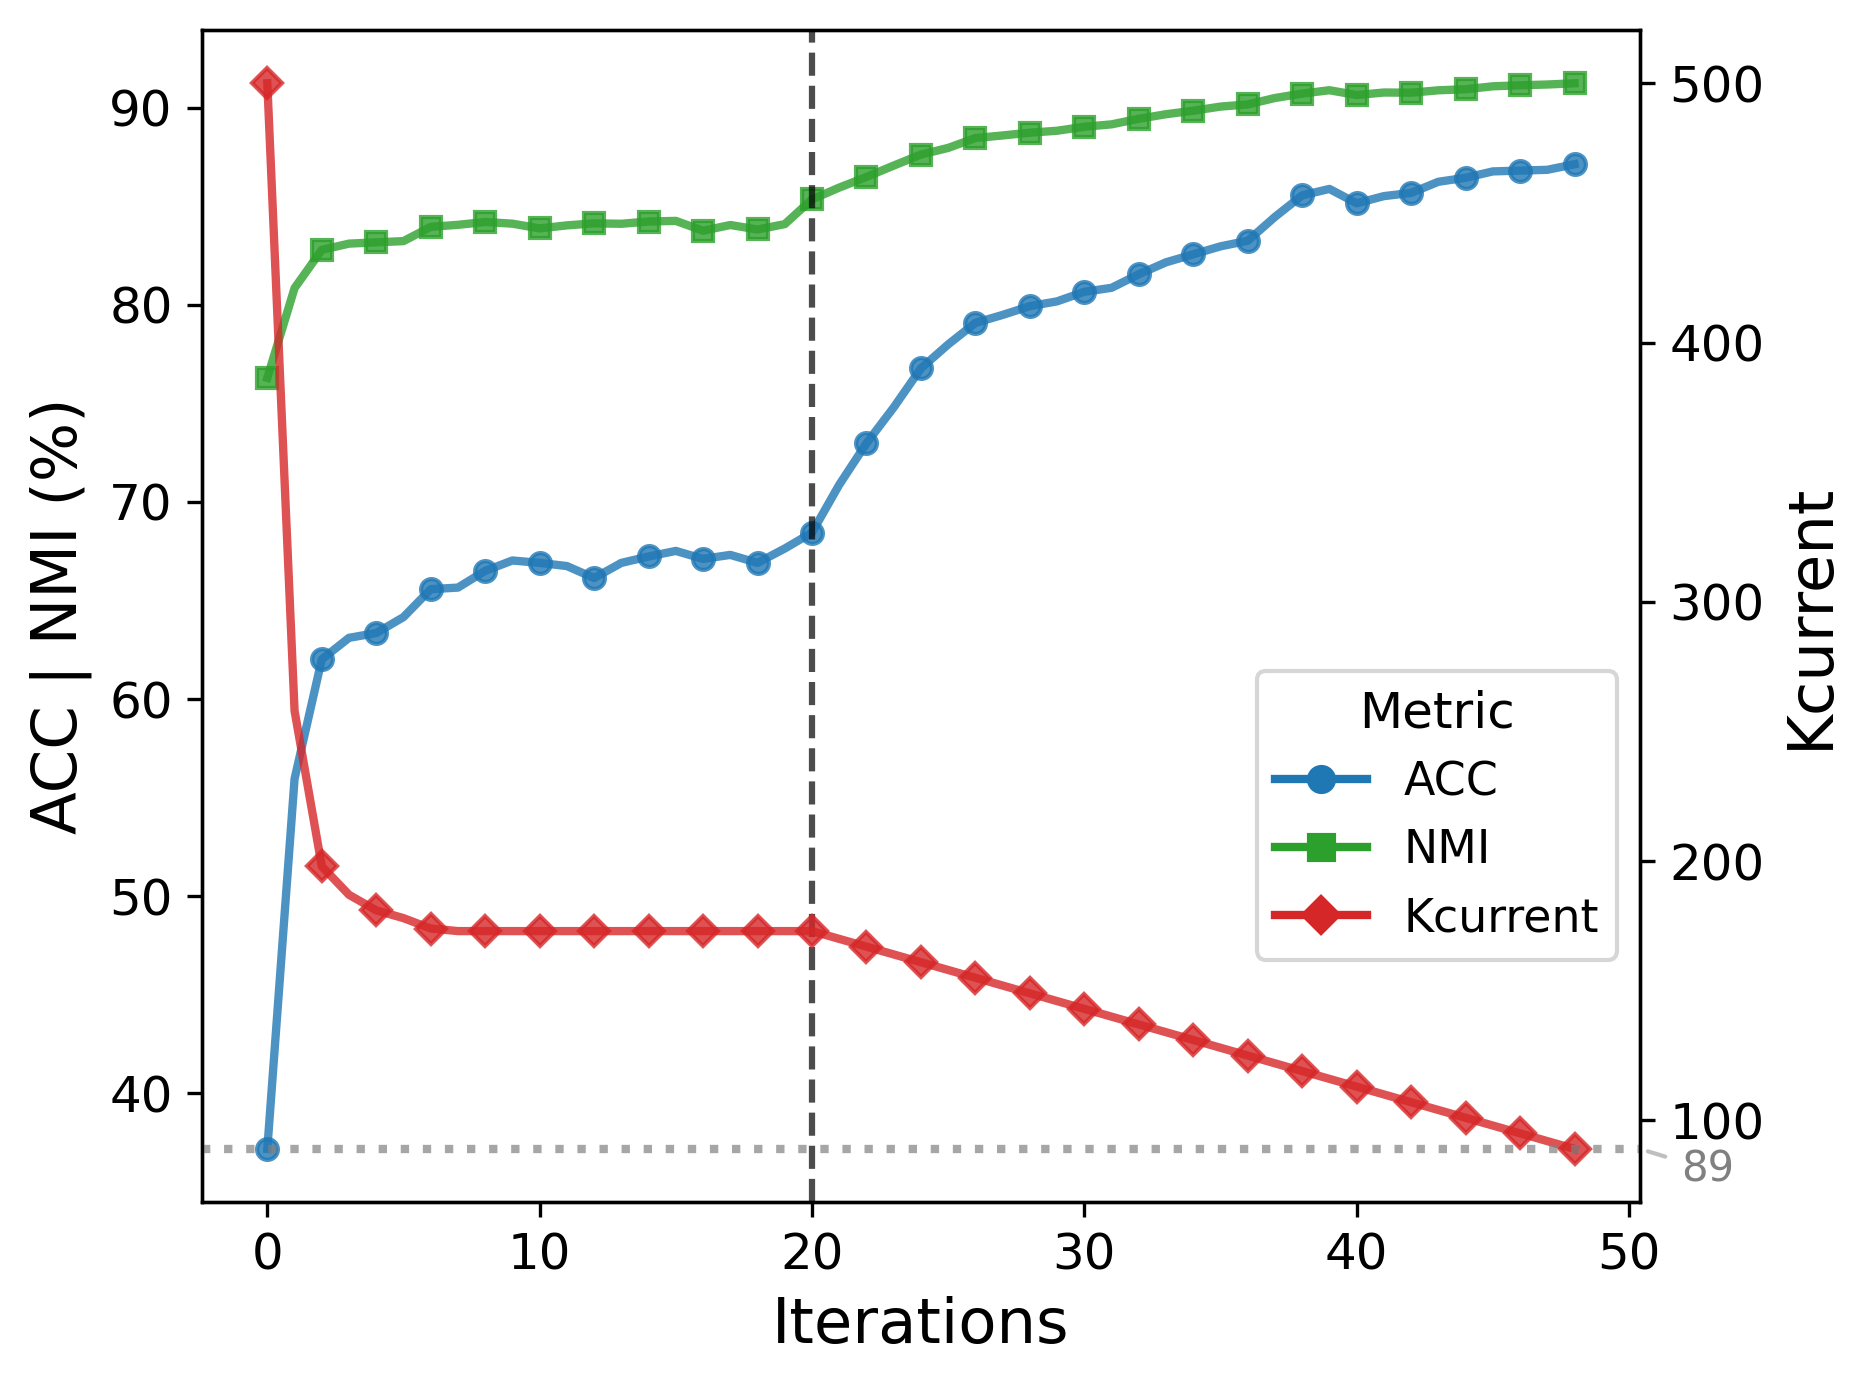
\includegraphics[width=0.98\textwidth]{figure/Tweet_tfIdf.png}}
\centerline{(a) Tweet}
\centerline{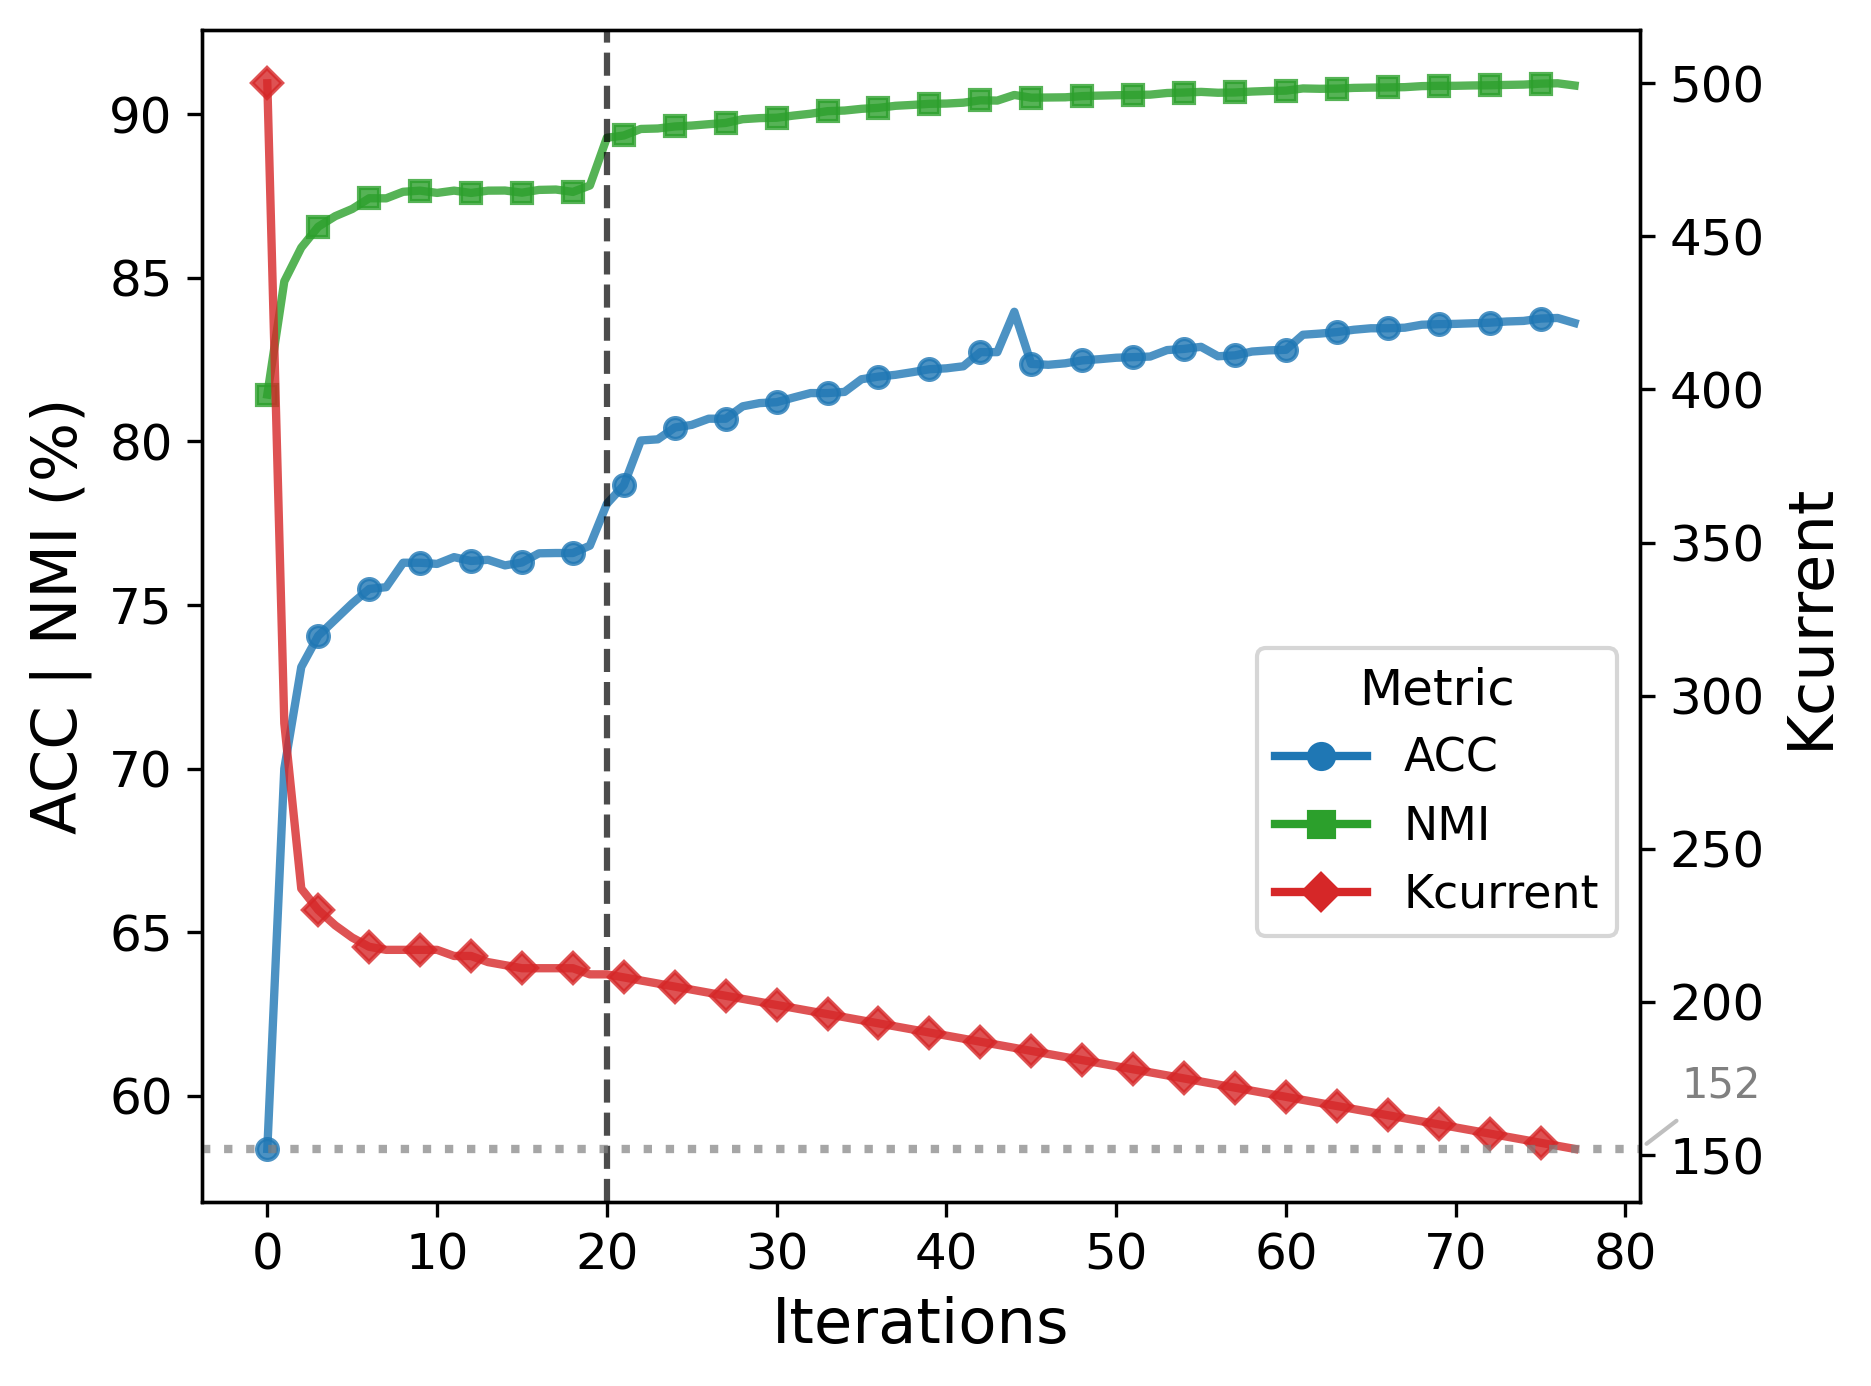
\includegraphics[width=0.98\textwidth]{figure/T_tfIdf.png}}
\centerline{(c) News-T}
\end{minipage}
\begin{minipage}{0.49\linewidth}
\centerline{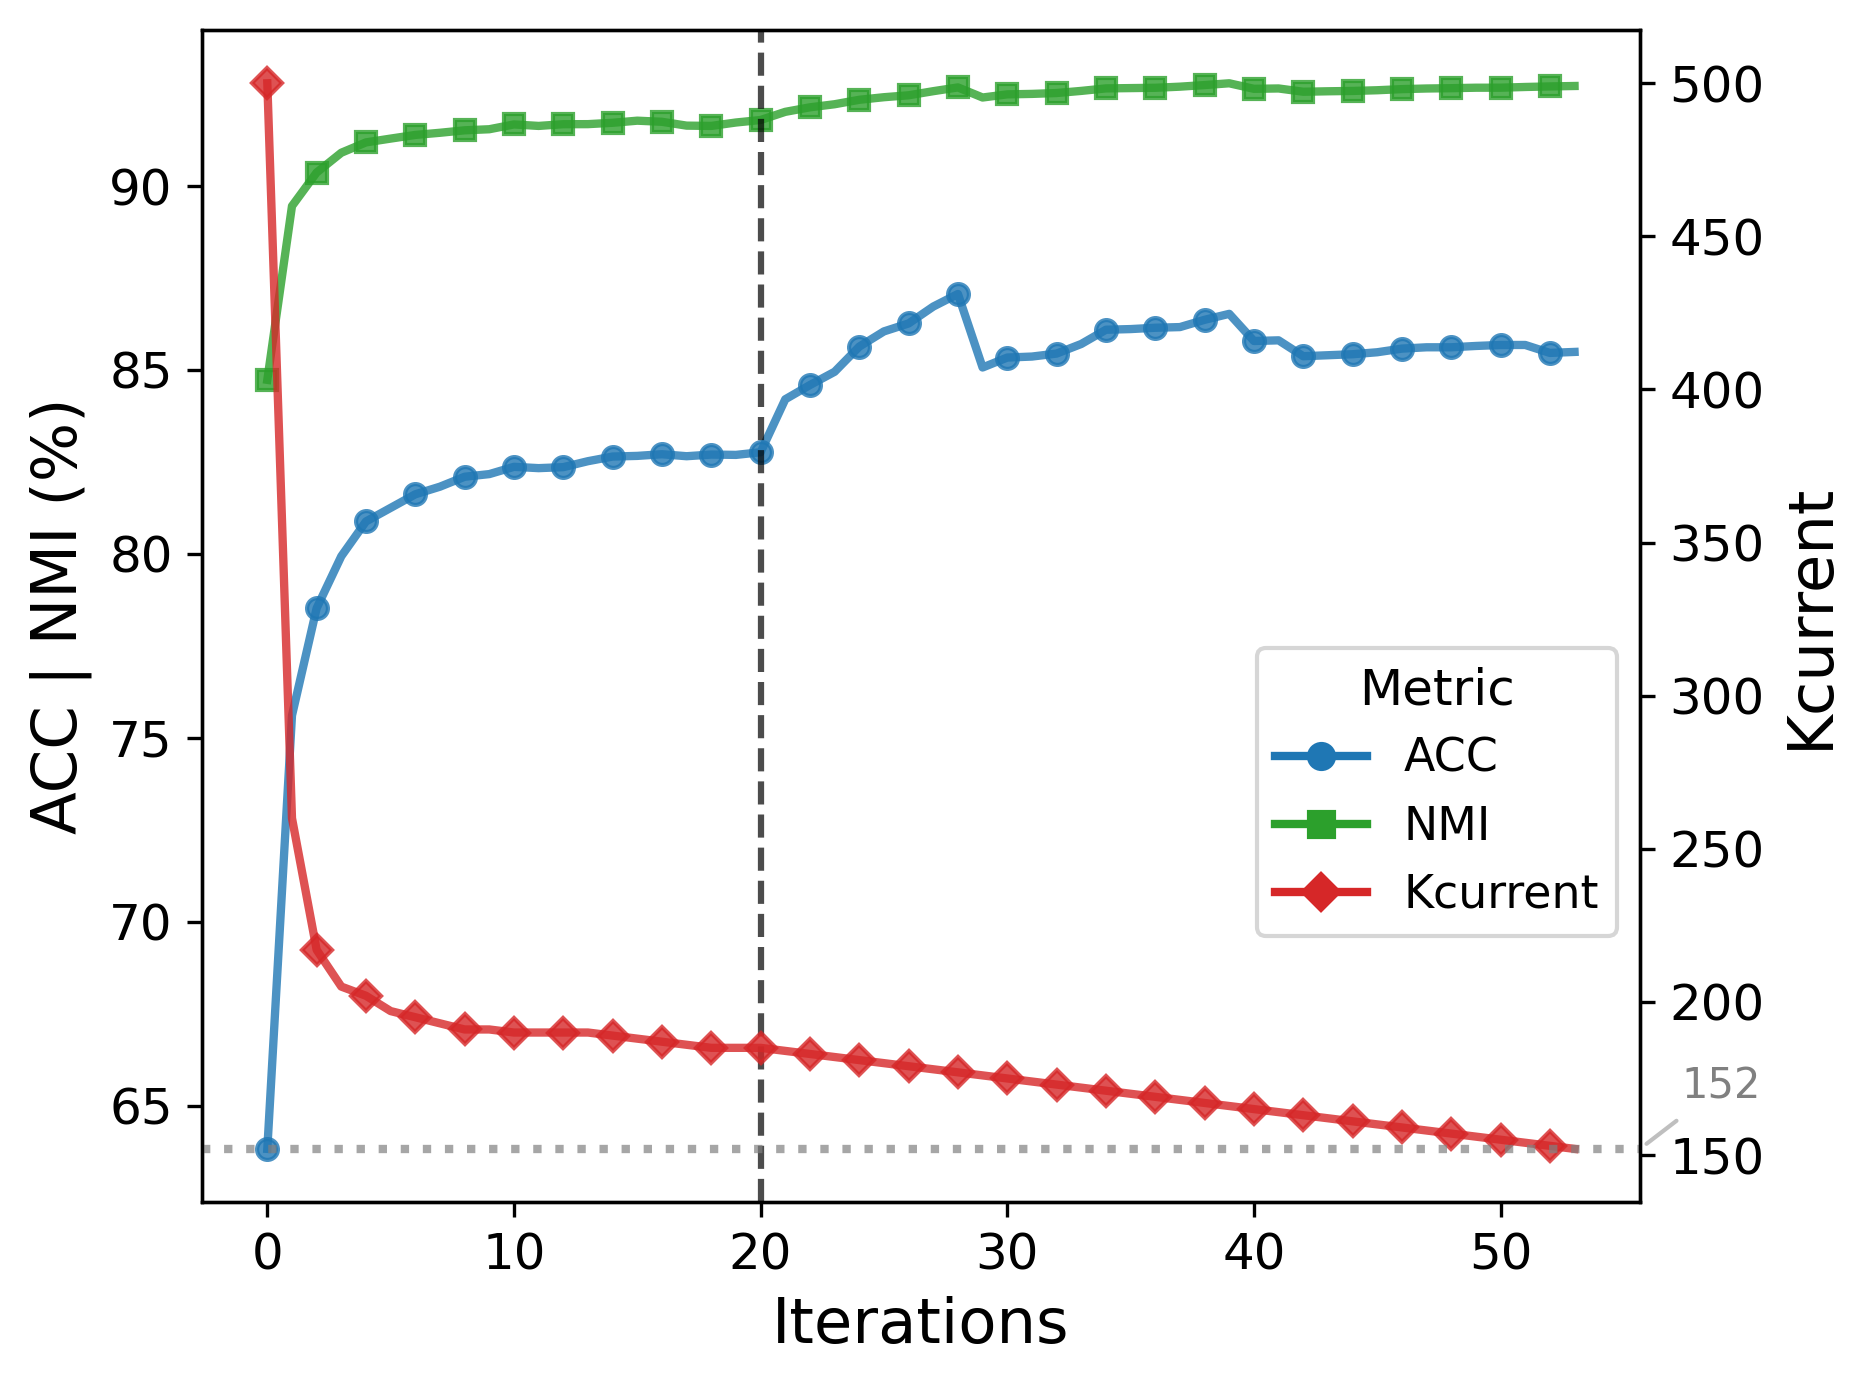
\includegraphics[width=0.98\textwidth]{figure/S_tfIdf.png}}
\centerline{(b) News-S}
\centerline{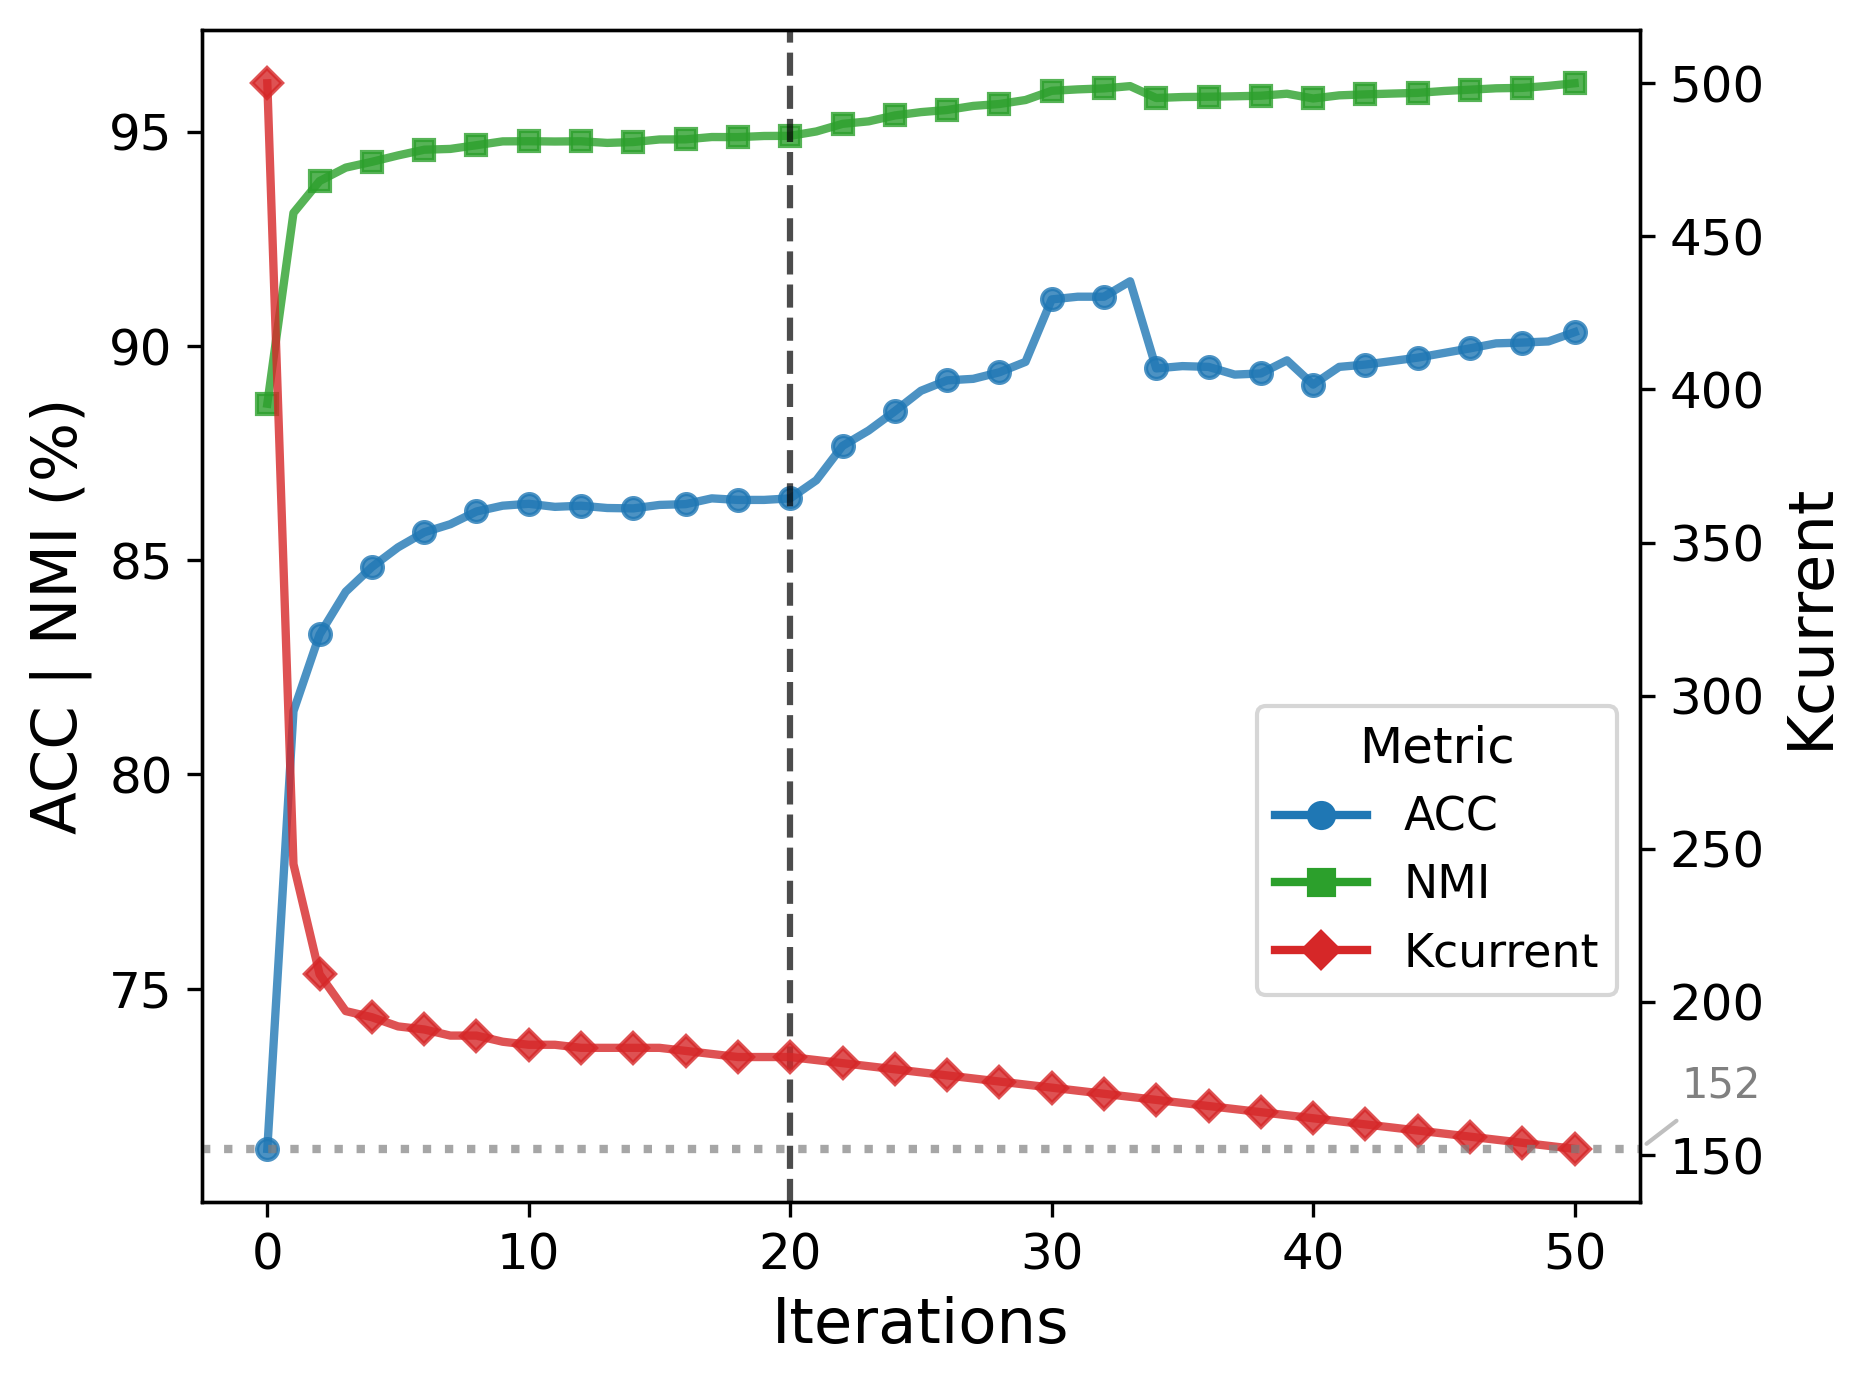
\includegraphics[width=0.98\textwidth]{figure/TS_tfIdf.png}}
\centerline{(d) News-TS}
\end{minipage}
\caption{The performance of \sysname{} over the iterations across four datasets, with vertical dashed lines in the figures indicating the beginning of granularity adjustment.}
\label{png_tfidf}
\end{figure}

Figure~\ref{png_tfidf} illustrates the clustering performance and the variation in the number of clusters across four datasets. The key advantages of this approach are twofold:
1) By iteratively refining the clusters through entropy-based updates, the model obtains more representative word distributions for each cluster. Although this leads to better separation of fine-grained semantic differences between clusters, it causes a deviation between the generated cluster distribution and the true cluster distribution. This design effectively adjusts the cluster granularity and eliminates the gap from the true number of clusters, delivering more accurate and meaningful clustering outcomes. 
2) Experimental results confirm that cluster merging significantly enhances the clustering performance. Compared to origin clustering approaches, cluster merging achieves a better balance between granularity and accuracy, leading to higher ACC and NMI scores.
